\documentclass[english,bachelor,a4paper,oneside,12pt]{ppfcmthesis}

\usepackage[utf8]{inputenc}

\usepackage[T1]{fontenc}
\usepackage[urw-garamond]{mathdesign}

\usepackage{amsfonts}
\usepackage{amsmath}

\usepackage{algorithm}
\usepackage[noend]{algorithmicplus}
\usepackage{listings}

\renewcommand{\tt}{\ttfamily}
\newcommand{\code}[1]{{\ttfamily #1}}
\newcommand{\PYG}[2]{#2}

\newcounter{tightListCounter}

% no extra spacing between lines
\newenvironment{tightList}[1][]
{
  \begin{list}{
                  \arabic{tightListCounter}.
              }
              {
                  \usecounter{tightListCounter}
                  \setlength{\topsep}{0.0em}
                  \setlength{\itemsep}{0.0em}
                  \setlength{\parsep}{0.0em}
                  \setlength{\listparindent}{0.0em}
                  #1
              }
}
{
  \end{list}
}

% Authors here.
\author{%
   Jan Kończak \album{84822} \and 
   Tomasz Żurkowski \album{84915}}
\authortitle{}                                        % Do not change.
 \title{{\Huge JPaxos} \hspace{5em} State~machine~replication based~on~the~Paxos~protocol}
%\title{JPaxos State~machine~replication based~on~the~Paxos~protocol}
 \titleNoFormat{JPaxos: State~machine~replication based~on~the~Paxos~protocol}
\ppsupervisor{dr hab. inż. Paweł T. Wojciechowski} % Your supervisor comes here.
\ppyear{February 2011}                                         % Year of final submission (not graduation!)

% commands here
\newenvironment{TODO}
{\begin{center}\par\noindent
{\huge \vspace{-3em} \par\noindent  \rule{0.85\textwidth}{0.1em}  \\ \vspace{-1em} \nointerlineskip
    \[ \mathbf{T} \, _\mathcal{O} \:\: \mathfrak{D} \, _\mathbb{O} \] }
    \begin{minipage}{0.8\textwidth}
}{\end{minipage} {\huge \vspace{-0.5em} \rule{0.85\textwidth}{0.1em}} \par\noindent \end{center} \par}

\newlength{\defaultParIndent}
\setlength{\defaultParIndent}{\parindent}

\newenvironment{minipageWithIndent}[1]
{
  \begin{center}
  \begin{minipage}{#1}
  \setlength{\parindent}{\defaultParIndent}
}
{
  \end{minipage}
  \end{center}
}

% Custom commands
\newcommand{\paragraphNewline}[1]
{
  \paragraph{#1} \hfill
  
  \noindent\ignorespaces
  %\paragraph{#1}
  %\par \noindent \par \noindent \ignorespaces
}
\newcommand{\paxosJava}[1][ ]{\textsc{PaxosJava#1}}
\newcommand{\alive}[1][ ]{\textsc{Alive#1}}
\newcommand{\prepare}[1][ ]{\textsc{Prepare#1}}
\newcommand{\prepareOK}[1][ ]{\textsc{PrepareOK#1}}
\newcommand{\propose}[1][ ]{\textsc{Propose#1}}
\newcommand{\accept}[1][ ]{\textsc{Accept#1}}
\newcommand{\catchUpQuery}[1][ ]{\textsc{Catch\-Up\-Query#1}}
\newcommand{\catchUpResponse}[1][ ]{\textsc{Catch\-Up\-Response#1}}
\newcommand{\catchUpSnapshot}[1][ ]{\textsc{CatchUpSnapshot#1}}
\newcommand{\proposer}[1][ ]{\textsc{Proposer#1}}
\newcommand{\acceptor}[1][ ]{\textsc{Acceptor#1}}
\newcommand{\learner}[1][ ]{\textsc{Learner#1}}
\newcommand{\recovery}[1][ ]{\textsc{Recovery#1}}
\newcommand{\recoveryAnswer}[1][ ]{\textsc{RecoveryAnswer#1}}


% From Nuno
\newconstruct{\INIT}{\textbf{Initialization:}}{}{\ENDINIT}{}
\newconstruct{\EVERY}{\textbf{every}}{}{\ENDEVERY}{}
\newconstruct{\UPON}{\textbf{upon}}{}{\ENDUPON}{\textbf{end upon}}
\newconstruct{\PROCEDURE}{\textbf{procedure}}{}{\ENDPROC}{\textbf{end procedure}}
\newcommand\BLANK{\SPACE}
\renewcommand{\mod}{\mathrm{~mod~}}


\usepackage{hyperref}
\hypersetup{% Set pdf properties
pdftitle = {JPaxos. State machine replication based on the Paxos protocol},%
pdfauthor = {Jan Kończak, Tomasz Żurkowski},%
pdfsubject = {JPaxos},%
pdfkeywords = {paxos} {state machine} {replication} {consensus} {recovery}%
 {atomic broadcast} {group communication} {reliable services},%
}

\begin{document}

% Front matter starts here
\frontmatter\pagestyle{empty}%
\maketitle\cleardoublepage%

% Blank info page for "karta dyplomowa"
\thispagestyle{empty}\vspace*{\fill}%
\begin{center}\strut\end{center}%
\vfill\cleardoublepage%

\thispagestyle{empty}\vspace*{\fill}
\vspace{10cm}
%\hspace{4cm}
\begin{flushright}\large\textit{We would like to thank our advisor dr Pawe\l{}
Wojciechowski,\\ for the opportunity to explore interesting areas of computer
science\\ and for the supervision of this work.}\end{flushright}%
\vfill\cleardoublepage

% abstract is already on ``karta dyplomowa''

% Table of contents.
\pagenumbering{Roman}\pagestyle{ppfcmthesis}%
\vspace*{-4em} \tableofcontents* \cleardoublepage%


% Main content of your thesis starts here.
\mainmatter%
\chapter{Introduction}

With the increase of usage and importance of Internet services in everyday life, there also increases demand on service reliability and constant availability.
Providing these features to the services is a complex matter, involving a trade-off between user satisfaction and service resource demands.

The most common and effective method of providing reliable services is replication. Applying the replication requires only minor changes for non-replicated service to become replicated one. Thus, this method is usable both for developing new services using well known design patterns as well as transforming existing services into replicated ones.

Each replication approach relies on some group communication mechanism, usually providing strong guarantees. For example, the total-order (atomic) broadcast is a very useful for interconnecting replicas -- it simplifies the design and implementation of the replication protocols, as it allows for dividing the system into two main modules with clearly visible responsibilities.

We have chosen to implement one of the replication approaches -- one that we think is very promising.
It is called active replication. In this approach, each replica does the same work. The replicas must behave identically and therefore we require the service to behave deterministically.

Every library for replicating services should address its main purpose, i.e.\ to guarantee high availability of service as well as durability of the service work results.


{\bfseries
As part of our diploma project, we have developed a library and runtime system for efficient service replication. Our system, written in Java, implements the Paxos protocol \cite{Lam98} for distributed consensus.

JPaxos requires deterministic behaviour from the service, does not tolerate Byzantine failures and works with static group of replicas.

JPaxos supports replica crashes as well as recovering the crashed replicas, \linebreak ensures durability in spite of failures, including the failure of all replicas at once. \linebreak It provides availability of service as long as a majority of replicas are correct.
}

\section{Thesis organization}

In the opening chapter we shortly characterize articles concerning Paxos algorithm and present the most significant definitions as well as theoretical results concerning Paxos.
The second chapter provides description of the Paxos algorithm.
In chapter 3 we describe the design of JPaxos -- its architecture, modules, important data structures and threading model.
Chapter 4 is devoted to the implementation work related to the state machine replication, including snapshotting, catch-up and achieving transparency for the service.
Fifth chapter contains description of optimizations we used in order to achieve better performance of the library.
Chapter 6 describes recovery related issues, both for Paxos and for the service replication.
The last chapter concludes the thesis.

\section{Related work}

The Paxos and MultiPaxos algorithms have been proposed by L. Lamport in \textit{The Part-Time Parliament}~\cite{Lam98}. Since the article presented the algorithm in quite specific form, the Paxos protocol has been described again by Lamport in \textit{Paxos Made Simple}~\cite{Lam01}.

Since then the Paxos protocol has been described from the theoretical point of view. Improvements and their proofs of correctness were presented as well as behaviour with byzantine crashes has been characterized.

One of the first real-world Paxos application has been described in 2007 (\textit{Paxos made live}~\cite{CGR07}). The article describes certain implementation issues concerning the Paxos algorithm in the Chubby distributed filesystem developed at Google.

A year later, in \textit{Paxos for system builders}~\cite{AK08}, the Paxos protocol has been described from programmer point of view.

In 2009, and subsequently in 2010, M. Primi et al.\ released two implementations of~Paxos designed to achieve good performance. Both of these implementations have been released as open-source. The first -- libPaxos$^2$ -- is described in Primi's master thesis, the latter -- RingPaxos -- is described in \textit{Ring Paxos: A High-Throughput Atomic Broadcast Protocol}~\cite{Mar10}.

The crash-recovery model has also been the subject of many research papers. \linebreak The \textit{Atomic Broadcast in Asynchronous Crash-Recovery Distributed Systems}~\cite{rodriguez2000atomic} provides definitions concerning recovery as well as shows a method to transform any crash-stop consensus protocol to the crash-recovery one.

A summary of the crash-recovery approaches for the Paxos algorithm can be found in N. Santos technical report~\cite{Nun10}. All algorithms implemented by us are described there.

\section{Contributions}

Jan Kończak has prepared the design and implementation~of:
\begin{tightList}
  \item[\textbullet] catch-up module (Section \ref{sec:catch_up}),
  \item[\textbullet] snapshotting module (Section \ref{sec:snapshotting}),
  \item[\textbullet] service proxy  (Section \ref{sec:serviceProxy}),
  \item[\textbullet] benchmark project.
\end{tightList}

\noindent Tomasz Żurkowski has prepared the design and implementation of:
\begin{tightList}
  \item[\textbullet] unit tests for JPaxos project,
  \item[\textbullet] client manager module, 
  \item[\textbullet] network module for communication between replicas,
  \item[\textbullet] view-based recovery (Section \ref{sec:view_ss}),
  \item[\textbullet] disc writers for full stable storage recovery.
\end{tightList}

\noindent JPaxos has been created in collaboration with Laboratoire de Systèmes Répartis at École Polytechnique Fédérale de Lausanne (Distributed Systems Laboratory at EPFL). Part of the ideas and implementations work has been done by Nuno Santos.

\noindent Nuno Santos has done:
\begin{tightList}
  \item[\textbullet] initial implemention of JPaxos
  \begin{tightList}
    \item[---] core MultiPaxos algorithm
    \item[---] failure detector and leader selection
    \item[---] basic replica, client and service implementation
  \end{tightList}
  \item[\textbullet] refactoring of batching and threading model
  \item[\textbullet] benchmarks of batching and pipelining modules
\end{tightList}

%\begin{tightList}
% \item[1.] Implementing, enhancing and fixing JPaxos
%  \begin{tightList}
%    \item[\textbullet] initial implementation 30.06.2009 (had about $13\%$ of current code size):
%    \begin{tightList}
%      \item[---] core MultiPaxos algorithm
%      \item[---] failure detector and leader selection
%      \item[---] basic replica, client and service implementation
%    \end{tightList}
%    \item[\textbullet] Renaming classes and cleaning up the code 22.09.2009
%    \item[\textbullet] Changing Benchmark project 06.10.2009
%    \item[\textbullet] Code cleanup 30.10.2009
%    \item[\textbullet] Tampering with the code 19.01.2010
%    \item[\textbullet] Improving the dispatcher thread 29.01.2010
%    \item[\textbullet] Moving failure detector from own thread to Paxos thread, tampering with the code 04.02.2020
%    \item[\textbullet] Adding support for paxos.properties file instead of hardcoded settings 05.02.2020
%    \item[\textbullet] Improving paxos.properties file 10.05.2010
%    \item[\textbullet] Code cleanup, theoretical bug fix 18.05.2010
%    \item[\textbullet] Moving catch-up from separate thread to the Paxos thread, rewrite proposer part batching, removing value from accept messages, improving retransmitter, rewriting TCP communication 22.06.2010
%    \item[\textbullet] Introducing priority queue in the Dispatcher thread, tampering with the code 24.06.2010
%    \item[\textbullet] Testing and fixes after branch merge 11.08.2010
%    \item[\textbullet] Improved batching 31.08.2010
%    \item[\textbullet] 'Improving' the TCP so that it does not work properly 30.09.2010
%  \end{tightList}
%
%  \item[2. ] Benchmarking and using JPaxos
%  \begin{tightList}
%    \item[\textbullet] Started Leader Oracle (not included in JPaxos) 22.09.2009
%    \item[\textbullet] Changes to Leader Oracle 22.01.2010
%    \item[\textbullet] Changes to Leader Oracle 04.02.2020 - 32.02.2010
%    \item[\textbullet] Modifications for improving benchmarks 07,15,26.07.2010
%    \item[\textbullet] Further improvements for benchmarks 17.08.2010
%    \item[\textbullet] Improving benchmarks again... 13.09.2010
%  \end{tightList}
%\end{tightList}


\noindent The remaining modules, benchmarks and bugfixes were the result of our joint work.


\clearpage

\section{Definitions}

In order to prevent misunderstandings and to clarify the subject of the thesis we begin from introducing
basic terms that we use in the reminder of this thesis.

\paragraph{Failure (crash)}
is a permanent lack of activity from a program. It may be caused by~programming error, lack of electricity etc.
We do not consider byzantine failures, i.e.~a~process may not misbehave in any way.

\paragraph{Catastrophic failure} is a failure of all processes at the same moment.

\paragraph{The failure model}
defines what type of failures can be tolerated by a system
\begin{tightList}[ \setlength{\leftmargin}{2\leftmargin}]
 \item[\textbf{Crash-Stop}] means that if a process failed, it failed permanently and must never be up again
 \item[\textbf{Crash-Recovery}] assumes that a crashed process may recover (i.e.\ start working again)
\end{tightList}

\paragraph{Correct process} is a process that did not crash, i.e.\ that works according to the expectations.

\paragraph{Consensus}
is a problem in distributed computing that encapsulates the task of reaching distributed agreement in the group of processes in the presence of faults.
The consensus protocol guarantees:

\begin{tightList}[\setlength{\leftmargin}{2\leftmargin}]
    \item[\textbf{Validity}] any value decided is a value proposed by some process,
    \item[\textbf{Agreement}] no two processes decide differently,
    \item[\textbf{Termination}] every correct process eventually decides,
    \item[\textbf{Integrity}] no process decides twice.
\end{tightList}

\paragraph{Instance (ballot)} is a single logical run of an algorithm. In order to decide on multiple values, many consecutive \textit{consensus instances} are executed, each identified by its \textit{ID}.

\paragraph{Value} is the value consensus agrees upon. In JPaxos, the value always consists of the client requests.

\paragraph{State machine}
is either a program, an algorithm or a protocol that can be described by its state and that can transit to other state only by receiving a command.
There are no restrictions how the state may change.

\paragraph{Deterministic state machine}
is a state machine that from the same state under the same command will always change state in the same way.
Thanks to this property, one may describe the state machine's state by the initial state and consecutive commands. 

\paragraph{State machine replication} is a method for implementing a replicated state machine, i.e.\ for maintaining multiple copies of identical state machine, possibly on separate network nodes, usually in order to gain availability of the state machine and durability of its state. State machine replication includes proper client handling and guaranteeing uniform state changes in all replicas.

\paragraph{Service}
is a program that receives requests (or commands) and executes them generating a response.

\paragraph{Deterministic service}
is a service that in a given state will always given the same response for a given command, and will always change its state to the same state.

\paragraph{Snapshot}
is the saved state of a service at a specified point in time that can be used by~the same service to restore its state to the exact state from the specified point in time. The snapshot should be in format that may be easily stored and transferred via network.

\paragraph{Client}
is the program sending requests to the service.

\paragraph{Atomic (total order) broadcast}
is a networking primitive providing send-to-all communication for which holds:
\begin{tightList}[\setlength{\leftmargin}{2\leftmargin}]
 \item[\textbf{Validity}] if a process delivers a message, it was broadcast by some process,
 \item[\textbf{Agreement}] if a process delivers a message, all valid processes will deliver it,
 \item[\textbf{Integrity}] a message is delivered only if it was broadcasted previously, and it reaches all valid processes at most once,
 \item[\textbf{Total order}] each two messages are delivered in the same order at every process.
\end{tightList}

\noindent The atomic broadcast problem is equivalent to consensus, i.e.\ if one can be solved, then the other also can be solved.

\paragraph{Stable storage}
is the memory that survives crashes. Usually stable storage denotes a~hard drive.
Sometimes also \textbf{volatile storage} name is used, to name memory that does not survive crashes, like the RAM memory.

\noindent The writes to the stable storage must be permanent contrary to the volatile memory. Thus if a hard drive is used, the writes must be synchronous.

\section{Theoretical limitations}

\paragraphNewline{The FLP impossibility result}

The consensus problem is not solvable in an asynchronous system where at least one process may crash and processes communicate by sending messages. This fact has been proved in the \cite{FLP}.

\paragraphNewline{Number of messages}

In the best case no algorithm is able to solve consensus faster than in the time needed to send one message with the value and one message not carrying value agreed upon.

Our implementation, as described in section \ref{par:bestCaseMessages}, is able to decide client commands in such time. Moreover, assuming that no network congestion occurs and no messages get lost the average time is equal to the best-case time.

However, with TCP and simple UDP it is not possible to use either multicast or~broadcast primitive; this prolongs the real time needed for sending a message, as~in the JPaxos network module \emph{broadcast} is translated to $n$ identical \textit{unicast} messages.

Other Paxos implementations do use a low-level multicast protocol for reducing communication. As an example, the RingPaxos \cite{Mar10} uses IP-multicast. The most significant gain from using multicast is scalability -- without the low-level multicast, each additional replica decreases the overall performance.


\chapter{Paxos}

In this chapter we provide some background for Paxos and MultiPaxos algorithm. We start with introduction to Paxos and MultiPaxos protocol. Then we describe the problems we encounter while implementing them and performance improvements we made.

\section{Overview}
Paxos algorithm is used to solve consensus problem in distributed system. $n$ processes tries to decide upon the same value, which was proposed by one of them. Paxos does not need a coordinator, however a processes may consider himself a leader for a certain time for specific ballot. As long as there is one leader and the majority of the processes are correct, liveness is guatanteed.

In order to simplify the Paxos as well as for increased preformance, MultiPaxos improvements proposed in \cite{Lam01} introduces one leader for all ballots.

The phase of electing the leader is described in following section. When the leader is elected, it starts proposing new values from clients.

\section{Leader Election}
\label{sec:leader_election}
\indent\par

To decide who is the current leader, our algorithm is using \textit{view} number. This number is sent in every message and processes keep track of the highest \textit{view} received. The current leader is a process for which \textit{view $\mod$ n $=$ local id}. For example, if \textit{view} = 5 and we have \textit{n} = 3 processes then processes with \textit{local id} = 2 is a current leader.

To detect if a leader is correct, failure detector is used. In JPaxos this is done using heartbeats sent periodically by the leader to all processes. The heartbeats are sent only when there are no other messages being sent, that is, the leader sends an \alive message to the replicas if it didn't sent any message during the last $\tau_0$ time.

When a replica does not receive a message from the leader for more than $\tau_1$ time, it suspects the leader and tries to become the new leader. This phase is called \textbf{prepare phase}. Process advances to the next view where it is the leader and sends a \prepare message to all. For example, if \textit{view} = 5, \textit{n} = 3 and we are process with \textit{local id} = 1, we will advance \textit{view} to number 7 -- first view where process 1 is a leader.

To become a leader, process needs to prepare the view. It sends the \prepare message to all processes with its new \textit{view}. Every process which received this message, advances its \textit{view} and responds with \prepareOK[]. When a process receives majority of \prepareOK message, it becomes a leader. Each \prepareOK message is a promise that the sender will drop all messages with lower view -- that means from old leaders or processes which do not know about the new leader.

\section{Propose Phase}

Every process keeps track of already proposed as well as decided values in a log. A log is ordered list of consensus instances -- triple \textit{<id, view, value>}. When a process is a leader, it can start a propose phase for new value. To propose a value, leader creates new consensus instance with first available id, current view and value to propose. Then it is send to all processes in \propose message. Every process by receiving the \propose message saves it to local log and sends \accept message to all. When any process receives the majority of \accept messages, it marks the proposed value as decided. The value is then passed to upper layers, in JPaxos it is executed on the state machine.

\section{Division of responsibility}

As introduced in \cite{Lam01}, the Paxos protocol tasks can easily be divided into three groups:
\begin{description}
 \item[Proposer] is responsible for proposing the values in correct order. In JPaxos it takes the requests from Replica and proposes them.
 
 \item[Acceptor] is a part of JPaxos that receives the \propose messages and responds to them according to the Paxos protocol -- that means responds if the view is not lower than current view.
 
 \item[Learner] gathers the \accept messages and if it gets the response from majority of acceptors, it marks the value as decided. In JPaxos, it informs the Replica that a decision has been taken.
\end{description}

Our implementation also uses this division in order to make the code more readable. Every process acts as acceptor and learner, and the leader also as proposer.

\section{Concurrent instances}
\label{subsec:concurrent_instances}
Running multiple consensus instances simultaneously is an easy way of making the MultiPaxos algorithm faster. Usually, single instance at time is not able to use available bandwidth; running more makes it possible to use the network more efficiently.

Theoretically, we may have any number of concurrent instances active at the same time. We can execute some decision only after all decisions from all instances with lower number have been executed.

In practical approach, the number of instances must be bounded due to following reasons:
\begin{itemize} 
  \item after leader change, \prepareOK must contain all leader's undecided instances,
  \item network has limited bandwidth, and conducting more instances will not increase throughput,
  \item there is no gain if we have decisions for some future instances, but the decision for an instance with lowest ID has not been taken yet (we can neither respond to the client, nor execute the taken decisions),
  \item using UDP, more concurrent instances are causing network congestion so packets are dropped by the system and instances are decided slower.
\end{itemize}

Biggest problem connected with concurrent instances is possibility of ordering the same request twice. Example scenarios explaining the problem:
\begin{figure*}[ht]
  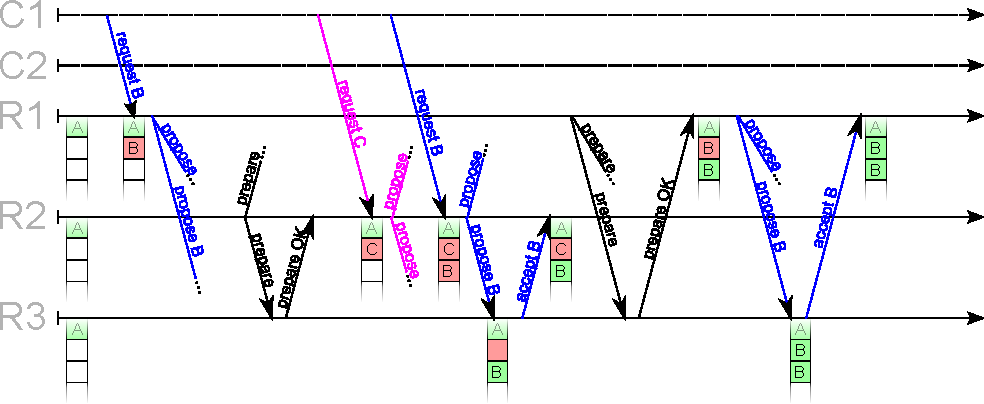
\includegraphics[keepaspectratio, width=\textwidth]{paxos/duplicating_messages.pdf}
  \caption{Duplicating messages - Scenario 1}
\end{figure*}
\begin{description}
  \item [Scenario 1] $R_1$ is the leader, proposes (1:B). No other processes receives these messages and $R_2$ becomes the leader. $R_2$ proposes (1:C) and (2:B). (2:B) is decided. $R_2$ fails and $R_1$ becomes the leader again. While preparing, it learns about (2:B). It has (1:B) as a previously accepted value. The Paxos algorithm requires $R_1$ to propose (1:B) again, since its the accepted value with the highest timestamp, but this will result in the request being decided twice.

  \item [Scenario 2] After a view change, the new primary will know about any value that might have been decided on a previous instance but it might not know about values that were proposed, accepted by up to a minority of replicas but not decided. Suppose that in instance $i$, process $p_1$ had proposed request $R_1$ which was accepted by a minority of replicas. The new primary, $p_2$ doesn't learn about request $R_1$ so it proposes no-op for instance $i$. More or less at the same time, the client resends the request $R_1$ to the new primary, which proposes it and gets it accepted as instance $i+2$, before the no-op request for instance $i$ being accepted. Process $p_2$ crashes and $p_1$ takes over again. Since $p_2$ didn't manage to get no-op accepted for instance $i$, $p_1$ proposes $R_1$ again which ends up being ordered both as instance $i$ and $i+2$.
\end{description} 

Unfortunately we cannot prevent instances from being decided twice in two different instances. Because of that, only valid solution for this problem is to remember last executed instance for every client and not executing them second time. But this requires to keep a new structure in memory as well as by every snapshot (after recovering from snapshot, this structure has to be loaded too).

Even if we cannot prevent from deciding request twice, we should minimise number of such situations because they slow down the algorithm (we have to send redundant data in each message). Possible solutions to decrease them are listed below:
\begin{itemize}
  \item We can cache last reply for each client, so after receiving the same request we can immediately response.
  \item Do not propose requests which are already decided
  \item Current leader can save which requested was proposed by him (but not decided yet) and also discard them. Because in \prepareOK message we can receive instance values which was unknown, leader has to deserialize them first.
\end{itemize}

\paragraph{Setting the window size}
The windows size specifies how many concurrent instances can be started (it has very similar meaning to window size in TCP protocol). In order to use available resources and keep high responsiveness window size must be set correctly. There is no global, generic solution: every usage needs different setting.

Most important thing is monitoring the network: its usage should be high -- but no congestion should occur.
That means, on one side, the window size must be enlarged as long as the links are not full, and on the other side, it must be guaranteed that no message will be delayed or dropped because of network traffic.

As long as these conditions hold, a speed of a single instance remains constant (putting aside CPU time).
If network is overused, the overall throughput may even stay on the same level, but the latency will increase for sure.

Notice that having future decisions instead of the present ones does not change decision count per time period, but causes inefficient task arrival time for state machine, especially if many of them arrive at the same time.

\paragraph{Performance Gains}
Single instance will nearly never use available bandwidth, so conducting concurrent instances will surely speed up JPaxos.

In full-duplex networks, concurrent instances will improve network utilisation, because when the leader is waiting for replies, the network from the leader to the followers is idle, so it can be used to send the next request. 

As already mentioned, this solution will improve latency and throughput. Carefulness is required in order to avoid network saturation, especially the link of the leader which has to carry $2n$ messages for each instance (as opposed to 2 messages for every other link).

\paragraph{Batching} is another method for improving performance and network usage. It is preferred over incereasing the concurrent instances count, however the benchmarks show that joining these two methods is better than any of them alone. Batching is described in section \ref{sec:batching}, as it does not concern the Paxos protocol, but values passed to the Proposer.

\section{No operation command}

The best method to understand the problem is to analyze the scenario below:

We have three replicas $R1$, $R2$ and $R3$. Replica $R1$ is the leader and proposes {1:A} and {2:B}. Value {2:B} was decided by all replicas, but {1:A} propose was lost. $R1$ fails and $R2$ becomes new leader. After preparing $R2$ has a gap in log because no information about instance 1 was received. 

As we can see after prepare phase, leader can have a gap in the log. Without filling this gap, replica cannot execute and propose new values. Because of that new value has to be proposed in this place.

With crash-stop or crash-recovery without stable storage the value may be lost forever. That happens when decision $n+1$ is already decided, and decision $n$ is unknown to all but leader, and the leader fails. As only he got the value, and it has been lost -- either because he is not allowed to recover, or he is recovering without stable storage.

On the other hand, the leader change may happen due to lost \alive message. In this case someone has the value, and it could be used back in the voting. But there is no simple and fast method to detect this situation.

The easiest solution is to create new request type called no-op, which is null operation and will be ignored by the replica. It fills the gaps, but is not executed on state machine.

\section{Log handling}

The replicated log cannot be allowed to grow forever, it must be bounded in any practical system. After any replica executes some command, it no longer needs the corresponding log entry locally. But other replicas may not have learnt the decision yet. In this case, these late replicas need to learn the decision by asking the corresponding log entry from a replica that still has it.

In JPaxos the Paxos protocol is not used for getting lost requests -- from performance reasons we use the process called \textit{catch-up}, which is described in section \ref{sec:catch_up}.

So having the old log is needed for view change and, in the crash-recovery model, for recovery.

Especially the latter is problematic. The view change requires always bounded number of instances in log. But if we assume recovery with minimal or no stable storage (as the Epoch based or View based ones), after the recovery a replica needs to recover the state from scratch. For this, it needs whole log -- or the state itself.

\paragraphNewline{Global Commit Point}

A command can be deleted from the log after being executed by all replicas in Crash-stop and Crash-recovery with stable storage models. The highest instance executed by all replicas is called \emph{global commit point}.

But the rule above is not enough to ensure that the log is kept bounded, because a correct replica may be disconnected from the system for some time. When communication is reestablished, the replica needs to learn about all the decisions taken in the meantime. If one replica crashes, the other replicas have no way of knowing that it is a crash and not a disconnection, so they would have to keep the logs forever. And the replica can stay crashed for arbitrary long time.

Therefore using snapshotting is the only acceptable solution in JPaxos.

\paragraphNewline{Snapshotting}

In order to be able to remove stale log entries snapshotting has to be implemented. It also speeds up the recovery and process of filling missing instances.

Upon reaching the limit of the log, new snapshot with full state is created and the old logs are truncated -- even if some other replica doesn't have them yet. When a replica that is missing old logs rejoins, most recent snapshot is transferred first, later all the decisions from the top of the log that were not yet applied to the state.

The size of snapshot is bounded, as the state machine must be implemented with the assumption of bounded memory, and the snapshot may be just the processes memory image. The size of the log is bounded as well -- we create new snapshot as log size reaches some limit.

The problematic part here is the Service -- if the JPaxos library user will not implement creating snapshots or will nor provide them often enough, the log will grow forever.

Snapshotting is described in details in the section \ref{sec:snapshotting}.

\section{Skipping redundant messages}
Reducing number of messages is one of the most efficient optimisation. In JPaxos we do not send messages to self, also the proposer doesn't send \accept messages.

It has been proven for Paxos consensus algorithm that it minimises the count of messages carrying value (client request in our case). The value is sent only once to each replica (not counting retransmission due to message loss). As for additional messages, their count varies among the certain implementations. Some of messages proposed in the typical implementation may be easily skipped without violating guarantees or adding assumptions.

\paragraphNewline{Sending to self}

As stated before, the Paxos can be divided into Proposer, Acceptors and Learners. Processes or some of their parts act as one of them. In order to communicate they must send messages to each other.

In our program every node consists of a (probable) proposer, acceptor as well as learner. In this case there is no need to send messages to self. Especially all send-to-all commands may be replaced by send to others command, as long as the communication with self will be done internally. This skips one \accept and one \propose sent by the leader, and one \accept by all other processes.

This does not influence the performance much, however it is recommended as it decreases system -- especially networking stack -- usage. It also skips a few system calls.

\paragraphNewline{Using {\normalfont\propose}as {\normalfont\accept}}

More important optimisation is merging the role of \accept and \textsc{Propose}. As long as acceptors and proposes do not share the log this is not allowed. But if their knowledge is identical and the leader proposed some value, then he must accept it as well. In most solutions one node acts as proposer and acceptor, and they do share the log.

So in JPaxos each \propose is simultaneously an \accept message. Notice that if the system consists of three nodes every process decides on the value by receiving a valid propose -- he knows that the leader and it itself accept the message. Normally the leader process has to send \propose to all first, later \accept to all. By this optimisation we are required to send the half of messages only.

This is a serious gain, clearly visible during benchmarks.

\paragraphNewline{Minimizing messages with value}

Most of the articles about Paxos state that the \accept message carries the value. This can be easily omitted.

Each processes in JPaxos waits not only for the majority of accepts, but before it sends the \accept message, it must receive a \propose with the value. So if a process accepts an instance, it already knows the value.

Waiting for another message might seem to cause additional overhead, but it makes JPaxos faster -- less network bandwidth is used by a single instance. Also usually the \propose will be delivered before any \accept message.

\paragraphNewline{Best-case messages}
\label{par:bestCaseMessages}

So, in normal operation in JPaxos:

\begin{tabular}{llllll}
          & Processes & Count & Time & Message  & Value  \\
 Proposer & $1$       & $n-1$ & $n$  & \propose & yes    \\
 Acceptor & $n-1$     & $n-1$ & 1    & \accept  & no
\end{tabular}

We can see that in order to decide we need to send once the \propose[], and later each not-leader process sends the \accept to others.

Other implementations consider using bounded learner count -- so that a acceptor sends \accept only to them. An additional message, \textsc{Decided}, is sent by learners to all as the ballot has finished. Thanks to this modification no reliable broadcast is needed, but also an additional phase must occur.

Interesting approach is presented in the RingPaxos (see \cite{Mar10}), where IP multicast is used for all broadcasts, what massively increases the scalability and performance.

\chapter{Architecture}

This chapter describes the architecture of JPaxos.
First the general architecture of the library is presented, consecutively focusing on its parts in detail.
Later the most significant data structures and the threading architecture details are presented.

\section{Architecture overview}
\indent\par
The easiest way to understand the architecture of JPaxos is to analyze its architecture in top-down approach.

\subsection{Processes and their communication}

For JPaxos there are two possible approaches of building replicated services. The first, recommended by us, 
requires from the service client application using a \texttt{Client} module. % TODO not English
The other approach incorporates the client module within replica, but 
it places the responsibility for finding a working replica on the user. % TODO rewrite
The possible approaches are visualised in figure \ref{fig:jpaxos_processes}.

% TODO enlarge
\begin{figure}[h]
 \begin{tabular}{ccc}
  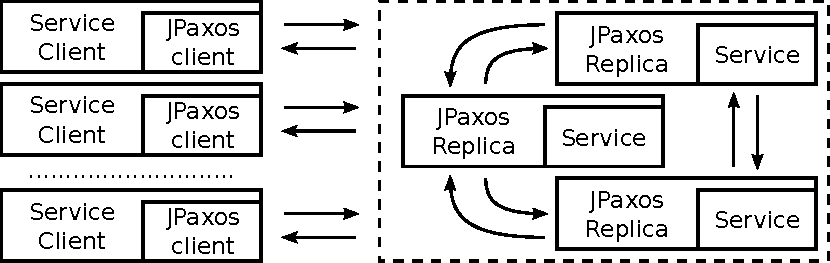
\includegraphics[width=0.44\textwidth]{architecture/userArchitecture1.pdf}
  &
  \hspace{0.02\textwidth}
  &
  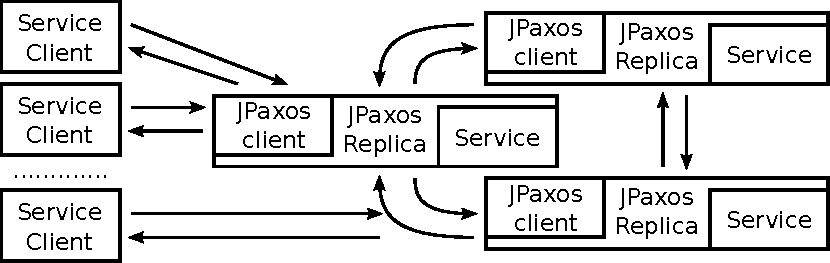
\includegraphics[width=0.44\textwidth]{architecture/userArchitecture2.pdf}
  \\ 
  \scriptsize a) JPaxos client integrated with service client
  & & 
  \scriptsize b) JPaxos client integrated with the replica\\
 \end{tabular}
 \fcmfcaption{Two models of JPaxos}\label{fig:jpaxos_processes}
\end{figure}

The JPaxos \texttt{Client} is responsible for connecting to replicas, providing availability of service as the replica connected with the client crashes, and ensuring that the request will be eventually answered.

Integrating the \texttt{Client} module with the service client provides full transparency of replication for the clients.
The service client contacts with the JPaxos \texttt{Client} module as if it would contact the service, i.e. it executes requests and gets answers for them.

If one chooses the second approach -- i.e. integrating \texttt{Client} in the replica, the transparency is lost, and the programmer must take care for selecting a working replica himself. However, this approach enables using JPaxos in a wider context. For example, one could possibly create a REST web service, and use a usual web client as the service client, while the service itself would be replicated using JPaxos.

The JPaxos Replica module is responsible for global request ordering, passing the requests to the service, answering to the clients and recovering service from crash.

The service itself must be integrated within JPaxos replica. Service gets the requests and returns the response. However, in order to make the resource usage bounded, JPaxos requires additional functionality from the service. This partially breaks transparency -- the service must provide periodically snapshots of it's state, as well as be able to recover it's state from a snapshot, possibly made by other replica.
As we assume that services are deterministic, recovering from snapshot originating from other replica is not a problem. However for some services creating a snapshot may present a challenge.

\subsection{Client and client-replica communication}

The JPaxos client module is a single, light-weight module that performs several tasks:

\begin{tightList}[\setlength{\topsep}{0pt} \setlength{\partopsep}{0pt}]
 \item[\textbullet] Connects to the replicated service
 \item[\textbullet] Reconnects automatically to the replicated service if the connection is lost
 \item[\textbullet] Retrieves (or acknowledges) a client ID for recognising the requests
 \item[\textbullet] Sends the requests
 \item[\textbullet] Waits for answer, retransmitting the request if needed
\end{tightList}

\noindent For the communication with replicas, the client module uses TCP protocol.

\subsection{Service}

% TODO More information about service, service proxy, service interface, service module

The Service module is the core part -- in fact it is the service that uses JPaxos for replication.
In order to integrate a service with the library, it must implement an interface specified in JPaxos. The interface provides required communication between the library and the service.

The interface for interconnecting JPaxos replica and service allows for:
\begin{tightList}
 \item[\textbullet] Executing requests and providing answers for them
 \item[\textbullet] Creating snapshots
 \item[\textbullet] Recovering from snapshots
\end{tightList}

\subsection{Replica}

Replica is the most important part of JPaxos. It consists of numerous modules as depicted in figure \ref{fig:replica_architecture}.

\begin{figure}[h]
 \centering
 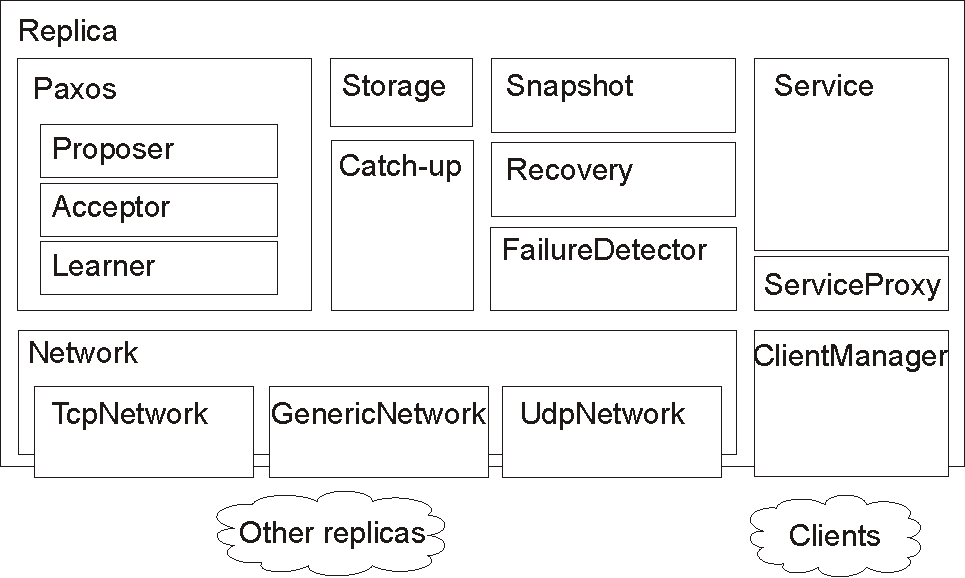
\includegraphics[keepaspectratio, width=0.75\textwidth]{architecture/replica_architecture.pdf}
 \caption{Block diagram of JPaxos modules}
 \label{fig:replica_architecture}
\end{figure}

Short description of the JPaxos modules goes as follows:

\begin{description}
  \item[Replica ] interconnects other modules -- especially the ClientManager, Paxos ans ServiceProxy
  \item[ClientManager ] maintains connection to clients, receives requests from them and forwards the answers
  \item[Paxos ] implements the MultiPaxos consensus algorithm
  \begin{description}
    \item[Proposer ] sends new proposes
    \item[Acceptor ] receives proposes and accepts them
    \item[Learner ] collects accepts and decides
  \end{description}
  \item[CatchUp ] takes care for lost ballots and retrieves the state from others on recovery
  \item[SnapshotMaintainer ] controls the snapshot mechanism
  \item[Recovery ] chooses a proper recovery method and does the actual recovery processes
  \item[Storage ] keeps the state of the Paxos protocol, i.e. view number, log of consensus instances and a snapshot
  \item[Service Proxy ] contacts with the user defined Service, provides as much trans\-pa\-rency as possible for the service
\end{description}

\section{Storage and data structures}
\label{sec:storage_and_data_structures}

Apart of modules and interaction among them it is important to choose proper routines to access data. Both within modules as well as data shared across whole JPaxos.% TODO not English

\subsection{Process descriptor}

Every application has some configurable options that stay unchanged during the run. In JPaxos all these constants are kept in the \texttt{ProcessDescriptor} class.

During the system startup, JPaxos reads a configuration file and initializes ProcessDescriptor with proper values for:
\begin{tightList}[\setlength{\labelwidth}{0em}]
 \item[\textbf{crashModel}] the crash model (see chapter \ref{chapter:recovery})
 \item[\textbf{logPath}] path for the stable storage
 \item[\textbf{localId}] the number of replica % TODO
 \item[\textbf{numReplicas}] count of the replicas % TODO
 \item[\textbf{windowSize}] a preferred window size (see \ref{subsec:concurrent_instances})
 \item[\textbf{batchingLevel}] a maximum size of the batch (see \ref{sec:batching})
 \item[\textbf{maxBatchDelay}] delay for connecting requests for batching in milliseconds
 \item[\textbf{network}] network protocol to be used (TCP or UDP)
 \item[\textbf{maxUdpPacketSize}] a threshold for generic network
\end{tightList}

\subsection{Storage interface}
\label{subsec:storage_interface}

\texttt{Storage} interface is responsible for holding the data for the Paxos protocol.

The data is shared across various modules.
It is very likely that various threads might want to access the \texttt{Storage} simultaneously. In order to prevent concurrency-related errors only one thread, the Dispatcher, may access these data. So if one wants to modify the \texttt{Storage}, a proper \texttt{Runnable} must be passed to the Dispatcher for execution (see subsection \ref{sec:threads}).

\paragraph{\normalfont \ttfamily Storage}
holds the data as follows:
\begin{tightList}[\setlength{\labelwidth}{0em}]
  \item[\textbf{log}] the Paxos Log (see section \ref{subsec:the_paxos_log})
  \item[\textbf{view}] current view
  \item[\textbf{firstUncommitted}] first instance not decided yet instance.
  \item[\textbf{windowSize}] the current size of the window used for multiple instances
  \item[\textbf{acceptors}] a list of processes acting as acceptors
  \item[\textbf{snapshot}] the most recent snapshot
  \item[\textbf{epoch}] the current epoch vector (see section \ref{sec:epoch_ss})
\end{tightList}

\strut

The type of \texttt{Storage} implementation must be chosen according to requirements impose by the model or recovery.
The implementation decides which elements must be kept in the stable storage and which may be placed in volatile memory.

\subsection{The Paxos Log}
\label{subsec:the_paxos_log}
The most important data structure for Paxos, the Log, is part of the \texttt{Storage}.
In our program responsible for that is the \texttt{Log} interface and the \texttt{Con\-sen\-susInstance} class.

\texttt{ConsensusInstance} is a class keeping all data related to a single instance of Paxos: % TODO
\begin{tightList}[\setlength{\itemindent}{0pt}\setlength{\leftmargin}{2\leftmargin}]
  \end{tightList}
  \item[\textbf{view}] a view of the last received message related with this instance,
  \item[\textbf{value}] the value which is held by this instance (i.e. packed requests that are received from clients and executed after deciding), %TODO deciding what
  \item[\textbf{state}] the instance can be in one of three states:
  \begin{tightList}[\setlength{\itemindent}{0pt} \setlength{\labelwidth}{7em}]
    \item[\texttt{\tiny UNKNOWN}] no information about the value of this instance,
    \item[\texttt{\tiny KNOWN}] a view and value are specified and \textbf{can} be changed later,
    \item[\texttt{\tiny DECIDED}] a value is already chosen and \textbf{cannot} be changed.
  \item[\textbf{accepts}] set of known replicas which acceptedthe (view, value) pair.
\end{tightList}

Theoretically \texttt{Log} should contain all instances from the first up to the current one. Of course, the implementation cannot provide this. The log must however contain all instances between the oldest still needed and current one. Only method that guarantees bounding the log (i.e. that count of needed instances will stay finite) is the ability to record a state of the Service periodically -- we call this functionality snapshotting (see \ref{sec:snapshotting}). % TODO rewrite

The \texttt{Log} implementation always keeps all instances with id between \textbf{lowestAvailableId} (inclusive) and \textbf{nextId} (exclusive). Instances below \textbf{lowestAvailableId} have already been truncated and instances above \textbf{nextId} are yet unknown. %TODO define lowestAvailableId

New instances can be appended to the log and after this operation \textbf{nextId} value is increased by 1. \\Log also allows to retrieve instances from it. There are three possible cases when retrieving an instance with a specified id:
\begin{itemize}
  \item (id $<$ lowestAvailableId) -- instance has been truncated and null value is returned,
  \item (lowestAvailableId $\leq$ id $<$ nextId) -- instance is inside log so it is returned,
  \item (nextId $\leq$ id) -- empty instances between nextId and id are created and an empty instance is returned.
\end{itemize}
Old instances can be removed by truncating the log and after that lowestAvailableId is increased. 

Appending, retrieving and truncating instances are three main operations per\-for\-med by log.

\subsection{Significant data structures}
% TODO is the Thesis reader able to understand what are these?
% it it information for the JPaxos "user" or "developer"? Or it's documentation of JPaxos design


Other noteworthy data structures include:
\label{subsubsec:significant_structures}
  \begin{description}
    \item[pendingRequests Map\textless RequestId, ClientId\textgreater] Keeps the requests received from the client for execution that were not yet executed. After execution of request, the reply is sent to client from this structure.
    \item[lastReplies Map\textless ClientId, Reply\textgreater] For each client, keeps the last reply that was sent to it. If client retransmits message which was executed, replica responses immediately.
    \item[decidedWaitingExecution Map\textless Integer, BatchedRequests\textgreater] Paxos might decide in\-stan\-ce $k$ before instance $k-1$, but the replica must execute all requests in order. So it must cache in\-stan\-ce $k$ until all previous instances are decided.
    \item[executedRequests Map\textless ClientId, Reply\textgreater] We have to save IDs of all requests which were executed on state machine to prevent executing the same request twice.
	\item[executedDifference Map\textless Integer, Replies\textgreater] Used to recreate executedRequests stru\-ctu\-re for moment when snapshot was made by state machine.
  \end{description}



\section{Threads}
\label{sec:threads}

A proper design of a multi-threaded application % TODO what application
must contain description of the major threads, their responsibilities and interactions. 

\begin{description}
  \item[Replica] \hfill
    
    Designed as an event loop. The thread % TODO what thread
    waits for new events at certain event queue and reacts on them.

    An event may either be a signal from Paxos about a new decision, or it may concern snapshotting, e.g. a new snapshot was made by service, the catch-up provided a new snapshot or a new snapshot has been requested from the service.

    For most of the time Replica thread waits for requests to be ordered. If they can not be executed yet, it puts them on a list (it uses for that % TODO ??
    the decidedWaitingExecution object).
    
    As for snapshotting -- the thread is a proxy ensuring linearizability in snapshot handling.
    Multiple threads (replica itself, dispatcher and catch-up) may therefore safely execute their snapshot-concerning routines.
    
  \item[Dispatcher] \hfill \nopagebreak
    
    Also designed as an event loop, the dispatcher executes the Paxos consensus algorithm as well as provides secure access to critical data structures -- to the \texttt{Storage} (see subsection \ref{subsec:storage_interface}).
    
    The Dispatcher thread is using a priority queue, so that the events are sorted by their importance -- for example, writes to the storage and the Paxos-related processing events have a higher priority than the Catch-Up tasks.
    
    The dispatcher is responsible for sending, receiving and handling most of protocol messages as well as accessing the \texttt{Storage} and triggering Catch-Up.
    
    Events are placed in the event queue in the following situations:
    

    % TODO methods? that generate these events or what?
    \begin{tabular}{rl}
      Recovery.NetworkListener & \begin{tabular}[t]{l}
                          received a new message \\
                          sent a message
                        \end{tabular} \\
      FailureDetector & \begin{tabular}[t]{l}
                          suspects another process \\
                          leader sends alive messages
                        \end{tabular} \\
      Paxos.NetworkListener & \begin{tabular}[t]{l}
                          received a new message \\
                          sent a message
                        \end{tabular} \\
      Paxos.propose() & \begin{tabular}[t]{l}
                          the application starts a new proposal
                        \end{tabular} \\
      Paxos.startProposal() & \begin{tabular}[t]{l}
                                the application asks the current process \\ \hspace{1em} to become a proposer.
                              \end{tabular} \\
      Proposer &  \begin{tabular}[t]{l}
                    timeout for requests to be batched
                  \end{tabular} \\
      Retransmitter & \begin{tabular}[t]{l}
                        message should be retransmitted
                      \end{tabular} \\
      Catch-Up &  \begin{tabular}[t]{l}
                   gets and merges log fragment \\
                   a message is received \\
                   received a snapshot form other replica \\
                   a periodcal catch-up should occur
                 \end{tabular} \\
      SnapshotMaintainer & \begin{tabular}[t]{l}
                             truncates the log after receiving new snapshot
                           \end{tabular} \\
    \end{tabular}


        % TODO What are these? (we should better describe what we want to present in this section and why)
	\item[NioClientManager] \hfill

		By using java.nio package, we only need one thread \textsc{SelectorThread} to manage all clients connection. Every time a new event occurs (an incoming connection waits for accepting, data received from client, data ready to be sent) an appropriate action is executed. The current implementation allows easy scaling % TODO ??
                to more \textsc{SelectorThread}'s to balance the CPU load if one thread wouldn't cope with a large number of connections.

	\item[UdpNetwork] \hfill

		One thread responsible for listening on DatagramSocket for datagram packages. Every time a new message is received, it is deserialised and all listeners are notified. 

	\item[TcpNetwork] \hfill

		For TCP connection between each two replicas a separate thread for receiving and transmitting is created. Also there is one thread which waits for new incoming connections. Overall we have  $2 \cdot \text{\textit{replica count}} - 1$ % TODO explain this in more detail
                threads handling TCP. Each of them can be in one of three states:
		\begin{itemize}
			\item connected, waiting for new messages,
			\item not connected, trying to establish a new connection,
			\item waiting for a new connection to be established by other replica.
		\end{itemize}
\end{description}

\chapter{Implemented Features}

In this chapter, we present the implementation details of some non-trivial modules.
We begin with our solution for differentiating the client requests. Later we describe the module responsible for keeping the replicas up-to-date. As next, we present the snapshotting mechanism in JPaxos. Last part of this chapter is devoted to improving transparency for the service programmer.

\section{Unique request IDs}

A request must be distinguishable from any other request. Only this guarantees that we will be able to say if a request is retransmitted, or it is a new one. A common method is to split the request identification in two parts: the client ID and a sequential number. As far as assigning a sequential number is trivial, a method providing unique client IDs must be chosen carefully, especially considering the crash-recovery model.

The client ID has to be unique for two different clients. To guarantee this, replicas must be responsible for granting IDs to clients, because a client has no knowledge of~other clients ID.

Below we present some of the possible methods for solving this problem:

\paragraphNewline{Based on the number of replicas}
Each replica can grant numbers incremented by a number of replicas, starting from ID of a local replica. For example, if we have three replicas, replica with ID 0 can grant numbers 0, 3, 6, 9, \ldots{} and replica with ID 2 can grant 2, 5, 8, \ldots{} . It guarantees that two different replicas will not grant the same ID. This solution works with the crash-stop and crash-recovery with stable storage. This will not work when replica can recover from crash without stable storage, because it does not know what was the last granted ID.

\clearpage

\paragraphNewline{Time based}
This is a different approach -- we use system time as the source of unique numbers. To~each client ID we also add information when the replica was started (in milliseconds).

For example, if a replica has been started at time $t$, it will grant to the new clients the following IDs: $(t + $\textit{localId}$)$, $(t + $\textit{localId}$ + n)$, $(t + $\textit{localId}$ + 2n)$ \ldots

This method assumes that the local system timer is not set back into past and also that the replica will not recover in the same millisecond. If these assumptions are fulfilled, then unique IDs are guaranteed also in the crash-recovery model without stable storage. This approach is currently set as default in our library.

\paragraphNewline{View-based}
Because time-based assumptions sometimes cannot be guaranteed, another approach for the crash-recovery model may be considered. Instead of adding information about start time, we can add the current view number. In each view, there is exactly one leader -- so after the prepare phase this replica can grant clients IDs as pair (view, sequence number). Two different replicas cannot start the same view.
Also, we have to guarantee that only the leader replica after prepare phase can grant new client IDs.

\section{Catch-up}
\label{sec:catch_up}

\paragraphNewline{Motivation}

Paxos must guarantee that every valid process will eventually decide. To decide, the process has to receive a propose message and majority of accept messages. In network with message loss, it is possible that the propose message from the leader will be lost. The leader after receiving majority of accept messages, will send next proposals and will never retransmit the lost propose again. Without the missing instance, the process is not able to execute any future instance.

Most papers about Paxos state that if a replica notices the lack of activity for some instance, it must send a new proposal and eventually decide. However, by using view for all instances, this would mean often view changes -- and this contradicts performance.

Therefore, a different approach is used by us -- a catch-up mechanism. The catch-up mechanism is using following observation -- if the leader is correct, and no activity about an instance is noticed, that means the value is already decided. The process with missing instance can ask the leader process about the decision for the instance. This solution \linebreak is faster than restarting the decided ballot and it does not require a view change.

\paragraphNewline{Recovery}

Catch-up module is also used by recovering the replica -- as a tool for downloading all decided instances up to the required state.

However, there is one drawback of using catch-up in recovery -- for the recovery, process needs to know also instances yet undecided.  However, if the system is operational, after a short time all required instances would be decided. If the system  is not operational, the recovery cannot converge. So downloading only decided instances is correct, but may cause small delay on recovery.

\subsection{Log-based vs state-based recovery}
\label{subsec:log_based_state_based_recovery}
A replica can catch-up either by copying the missing decisions or by a combination of transferring the state plus the most recent decisions.

In the rest of this paper \emph{log-based recovery} refers to the first option while \emph{state-based recovery} refers to the second option.

One should use of course the method achieving better performance. However, which method is faster depends on the particular characteristics of the system:

\begin{description}
  \item[Size of the state] For services with large states  it is better to avoid transferring the state as much as possible. On the other hand, if the service state is small, transferring it might be better. In the extreme case, the service state is of a similar size or smaller than a single command. In this case, it would always be better to transfer the state.

  \item[Execution overhead] Executing commands takes some processing time which is not required when transferring the state. Therefore, even if the service state is bigger than the corresponding commands, it might be faster to transfer the state.

  \item[Bandwidth available] With limited bandwidth, the fastest  method will likely be the one that transfers less data. Otherwise, the execution overhead will likely be the dominant factor.
\end{description}

\paragraphNewline{State-based recovery time}

State-base recovery has the following steps:

\begin{center}
  \begin{tabular}{ll}
    Serialization               & state is transformed into a sequence of bytes \\
    Transfer                    & state is sent via network \\
    Deserialization             & state is rebuilt at destination \vspace{0.5em} \\
    Residual log-based-recovery & recovery from snapshot process is made \\
  \end{tabular}
\end{center}

The first three tasks may be done concurrently. If the fourth task is comparatively fast, we can consider that the total recovery time is the maximum time it takes to do each of the first three tasks.

\paragraphNewline{Log-based recovery time}

Log-based recovery is done by sending the commands and executing them at the replica. Once again, sending and executing can be done concurrently, so the total duration is the max of the time it takes to transfer all the updates or to execute them.

\subsection{Conditions for starting and finishing the catch-up}
\label{subsec:conditions_for_starting_and_finishing_the_catch_up}
Many possible rationales may be used as indicator when the process should begin the catch-up. In addition, conditions needed for the stop process are a significant issue.

\paragraph*{Starting catch-up}
Activating the mechanism should not happen too early, that is when Paxos itself is still able to take the decision -- target of catch-up is to complement decisions missing due to packet loss. On the other hand late initiating leads to delaying command execution, and thus significant performance loss.

Most common events used to initialize the algorithm are:
\begin{itemize}
  \item No traffic for the ballot during a particular period of time (\textsc{timeout})
  \item An instance with higher ID (i.e.\ newer instance) has already been decided \\ (\textsc{higher instance decided})
  \item Instance with ID higher than $\alpha$ has been started, and the implementation ensures that only instances up to $\alpha$ are started as $\alpha-ws$ stays undecided (\textsc{window})
  \item Activate periodically the mechanism (\textsc{periodical})
\end{itemize}

These methods let the replica suspect, that a locally undecided instance has already been decided, so its log state is not up to date. It is good to use more than one of them, as each method is sensitive for a particular scenario, perhaps performing bad otherwise.

Simplest, but not efficient for most uses is the \textsc{periodical} method -- it guarantees that from time to time the replica will be up to date.
However the method used too often may cause bandwidth and processor consumption, too rarely -- having old state for unacceptably long time.

The \textsc{timeout} event is caused either if problems with network occur, or if the \accept messages were lost -- otherwise current leader and other replicas would generate traffic for the ballot. The replica should try to learn the state of voting in such case, otherwise as long as no new proposal will arise the replica will have an old state.

\textsc{higher instance decided} means that a voting started later has already finished. We may assume the previous voting took similar amount of time -- that is, it should be already finished. Message loss or varying latency can also cause the situation that a newer consensus is decided as the older is still in progress. To avoid the situation the method may be extended to: if the number of newer decided instances exceeds a~constant value, then the catch-up should be initiated.

This method, as well as the method described earlier, may be used in case when operations on state machine require long processing. The risk of loosing small bandwidth for catch-up may be small enough compared to earlier arrival time of resource-consuming task.

The \textsc{window} method is very useful because of its assumption: the algorithm uses a~window of the maximum size $ws$. If the condition that all decisions outside the window must be decided is violated on one replica, it means that the other replicas, at least the current leader, have already decided the instance. This means no new messages concerning the ballot will emerge, and catch-up is necessary.

A different problem is when a replica does not know that the instance already exists (for example, a short-time netsplit or bad luck caused all messages for the replica to be dropped). In this case, the catch-up should be started as well. 
Either periodic request must be sent, or additional information must be acquired. It should be emphasized, that as any newer ballot starts, the replica is informed about the existence of missing instance.

Although this is not critical, it prevents state machine from executing the command until a new instance emerges. That means performance loss, as the old command must be caught-up and executed before the new.

In our system, replica is notified about the highest instance ID from the \alive message from the leader. The leader is attaching this number to every \alive message sent. This guarantees that every replica learns what instances already exist within the failure detector timeout.

\paragraph*{Stopping catch-up} As the algorithm runs, the state of Paxos may not be stable, \linebreak i.e.\ new ballots may start. Therefore selecting the moment when catch-up should be deactivated is not trivial.

One method is to calculate conditions a priori (for example the IDs of missing instances), and continue the process as long as needed. However, this can easily lead to constant switching on and off the catch-up -- voting for new instances may be faster than catching up, so as the predefined conditions are met, new event already caused catch-up activation.

The better solution is to determine dynamically if catch-up is still needed. A method that seems most convenient for that is checking if all instances outside the window are already decided. Stopping earlier is bad, as we know that at least the current leader must have decided for the missing instances, and that means we will not get the value via the Paxos algorithm.

Finishing the catch-up process later, that is requiring any messages in the window to be decided, is also not a good solution -- unless we have some additional knowledge that the instance has already been decided (for example, the leader's last uncommitted instance ID is sent in \propose or \alive messages).

Problem arises, if there really were decided instances inside the window. If there are no new ballots, arrival time of these requests will be delayed. In our opinion, the problem is not that severe, especially if the window size does not exceed reasonable size.

\subsection{Transport protocol}
\label{subsec:transport_protocole}
As very separate from Paxos, the catch-up may use a different transport protocol than the consensus algorithm.
Choice of the transport layer must take into account the characteristics of this mechanism as well.

Both TCP and UDP may be used -- both having their pros and cons, presented in~table~below:

\begin{center}
  \begin{tabular}{m{0.47\textwidth}|m{0.47\textwidth}}
    \multicolumn{1}{c|}{ \textbf{TCP} }                          & \multicolumn{1}{c}{ \textbf{UDP} } \\ \hline
    automatic retransmission guaranteed by protocol             & retransmission must be implemented manually \\
    flow control provided by protocol                           & no flow control, it \emph{is} easy to congest network \\
    big messages automatically fragmented, mer\-ged and managed & splitting and handling big messages must be~self implemented \\
    request cannot be changed at retransmission                 & request can be changed each retransmission \\
    default retransmission time                                 & custom retransmission time \\
    another message may be sent once the previous was delivered & new datagram may be sent anytime, no matter if the previous reached the target \\
  \end{tabular}
\end{center}

When catch-up is needed, our network must have (probably high) message loss. That means the catch-up messages may also get easily lost.

We have noticed, that it is more efficient to use UDP for all smaller messages -- if the package gets lost, we are retransmitting it with updated query. Sometimes a UDP message retransmitted even twice reaches its target faster then the same message sent with TCP. In TCP, the timeout for the ACK message grows automatically -- and that may cause big delays. During experiments, with 30\% message loss, transmitting a message using TCP that is smaller than the UDP-datagram size took even more than 4 seconds to reach the other side.

In UDP, a single message delay or loss does not block the communication to the replica -- but in TCP, it does.
In this case, no new catch-up query may be sent to this replica, as long as the previous will be processed. The request cannot of course be changed. It~means that once we got the response, the core protocol may have already missed another instances to catch-up.

\subsection{Requirements}
\label{subsec:catch_up_requirements}
The speed and the resource consumption must be correctly balanced.

In theory, catching-up can be delayed any finite time. On the other hand, it is important for the view changes and for bounding the size of the log. A view change will take longer if the new leader is missing many requests. Since during a view change no new requests are being satisfied, we need to keep its length as short as possible. Additionally, if a replica does not know the instance $i$, it cannot execute any request higher than $i-1$. This also means that it cannot remove entries from the log.

In practical approach, most significant requirements for catch-up are: good performance and small resource usage. For sure catching up should not slow down the core protocol.
Good performance demand has one main reason: the arrival time of the tasks for the state machine is dependent on being up to date. If catch-up would get the information too late, the state machine would get long list of, possibly high CPU-consuming, tasks at once, instead of doing them in spare time before.

Therefore, it is desirable to run the catch-up mechanism as often as possible, but without slowing down the service significantly.

It should be noticed, that only the followers would have to catch-up, since the primary learns all previous decisions on a view change and then it is the one proposing new values and leading the protocol.

\subsection{Catch-up algorithm}
\label{subsec:catch_up_algorithm}
The catch-up algorithm should contact other replicas and copy the decisions that are not known. The question when this should be done is discussed in Section \ref{subsec:conditions_for_starting_and_finishing_the_catch_up}. Here the main idea of JPaxos catch-up algorithm is presented.

To activate the catch-up, we use \textsc{window} and \textsc{periodical} methods (see Section \ref{subsec:conditions_for_starting_and_finishing_the_catch_up}). The leader also sends in each \alive message the information about highest started instance.
This ensures that the replica will catch-up eventually, even if there are no new requests, and that a replica never stays too much behind the others, at most \textit{ws}.

There are three messages that may be sent during the algorithm: \catchUpQuery[], \catchUpResponse and \catchUpSnapshot[].
\begin{description}
 \item[\normalfont\catchUpQuery --] a request for missing instances. It carries a list of missing IDs and may have one of two flags set: the first flag indicates if this was a periodical catch-up, second one -- 
 if we want to get the last snapshot, not the missing instances.
 \item[\normalfont\catchUpResponse --] response sent for every received request. It has a list of decided instances for requested numbers. The list may be empty. This message may have two flags: periodical flag and snapshot only flag. The periodical flag is set if this is response to the periodical query. The snapshot only flag is set if the replica does not have an old enough instances, and transferring a snapshot is the only possibility.
 \item[\normalfont\catchUpSnapshot --] if another replica asked for snapshot, this message is sent with most recent snapshot.
\end{description}

The list describing missing instances is constructed by replica in straightforward way: it contains all undecided instance numbers plus the (highestID+1) as the first instance, the replica has no knowledge about. The responder sends therefore all decided instances from the list and all decided instances that are higher or equal the additional number.

In order to make the messages smaller, a trick has been used: the list contains two lists. One, called a range list and the other, an instance list.
The range list contains intervals we miss, while the instance list -- single numbers. For example, if we would miss instances 1, 2, 4, 6, 7, 8, 9, 11, and the highest instance we know is 12 (state decided) our lists would look like:
\begin{quote}
$[\langle1,2\rangle; \langle6,9\rangle]; [4,11,13]$
\end{quote} 
Notice the number 13 -- it is the first we have no idea of existing, as mentioned above.

Catch-up works as follows:

\begin{algorithmic}[1]
  \REPEAT
    \STATE \label{alg_1_a} Choosing target replica
    \STATE Creating list of missing instances
    \STATE Send a \catchUpQuery
    \STATE \label{alg_1_b} Wait for timeout or for response
  \UNTIL{\label{alg_1_c} catch-up succeeds}
  
  \vspace{0.5em}
  
  \STATE \textbf{upon} receiving \catchUpQuery \textit{query}
    \IF{\textit{query} has snapshot flag set}
      \STATE Get last snapshot
      \STATE Prepare \catchUpSnapshot message
      \STATE Send the message
    \ELSIF{requested instances already not in log}
      \STATE Send \catchUpResponse with \textit{snapshot} flag
    \ELSE
      \STATE Gather all decided instances
      \STATE Send \catchUpResponse
    \ENDIF

  \vspace{0.5em}
  \STATE \textbf{upon} receiving \catchUpResponse \textit{response}
    \IF{\textit{response} has \textit{snapshot} flag set}
      \STATE Prepare \catchUpQuery with snapshot flag
      \STATE Send the query
    \ELSE
      \STATE Merge received log (if any)
      \STATE Wake up the catch-up loop (line \ref{alg_1_b})
    \ENDIF
  
  \vspace{0.5em}
  \STATE \textbf{upon} receiving \catchUpSnapshot \textit{snapshot}
  \STATE Check if \textit{snapshot} is newer than current one
  \STATE Replace the current snapshot with \textit{snapshot}
  \STATE Truncate logs (to stop catch-up)
  \STATE Wake up the catch-up loop (line \ref{alg_1_b})

\end{algorithmic}

\vspace{1em}

In line \ref{alg_1_a} a best replica is chosen. We have implemented it as follows: a rating for each replica is kept. When sending a message, the rating decreases; when receiving response it rises. If an empty response is received (except for the \textsc{periodic} mode), we request asking the leader next time. The best replica for us is a follower with the highest positive rating, or the leader if all followers have negative rating.

The line \ref{alg_1_c} executes a predicate checking if the catch-up shall finish (see Section \ref{subsec:conditions_for_starting_and_finishing_the_catch_up}).

\section{Snapshotting}
\label{sec:snapshotting}
As presented before, the support of storing and transmitting state of replicated machine is a very useful and important part of a replica. In practical systems, it is necessary -- it allows log truncating, faster recovery and catch-up.

\subsection{When to snapshot}
\label{subsec:when_to_snapshot}
Snapshots are needed in two cases: to enable catch-up and recovery, and to truncate the log. For both uses there is a different \textit{best moment} for making snapshot.

As for recovery, we get the best recovery result if the snapshot would be done every executed order.
This, of course, is not the solution. It would completely decrease the throughput -- snapshot creation is resource-consuming.

For the catch-up the moment when another replica requests snapshot is the best for creating one. 
However some services cannot create snapshot anytime. So demanding a~snapshot from the service is not acceptable.

The snapshot should be created periodically to truncate the log without any additional requirements.

Therefore, we assume the snapshot should be made when the cost of catch-up from the log becomes bigger than the cost of catch-up from the snapshot.

Please note that catch-up time also includes time of state/log transfer.

\subsection{Replica vs service responsibility}
\label{subsec:replica_vs_state_machine_responsibility}
There are two approaches to the problem who is in charge for the initiating of snapshot creation. Either the JPaxos \texttt{Replica} module issues a snapshot, or the service chooses an~appropriate moment.

Embedding this functionality into JPaxos would surely provide more secure work (the service may simply not deliver the snapshots, which means forever growing log). It~is~easier for the \texttt{Replica} to measure the size of the messages that should be transferred in order to catch-up (or recover).

However, JPaxos does not know anything about the service. We can also assume, that the service is not aware of network conditions. Therefore choosing the proper moment (when the cost of log-based catch-up becomes more expensive than the state-based catch-up) is impossible for both. It is clearly visible, that service is better informed -- it knows not only the size of requests, but also it may estimate the size of its current state and the resources that are needed to execute all commands from the log.

The latter is most significant difference: JPaxos has no idea how long the log execution from previous snapshot would take. It seems possible to estimate this: measuring the time between a request and the reply to that request might solve the problem. However, such estimate can give mistaken results, especially in a multi-process environment. If another process is consuming CPU, or the replica waits a long time for granting some resources (like an access to a file or even a printer), the estimate surely will not reflect the real value.

Below we present a table showing in compact way the state of knowledge needed to~select the best moment for a next snapshot:

\begin{table}[h]
\small \centering
\begin{tabular}{r|c|c|}
\cline{2-3}
 & Service & JPaxos \texttt{Replica} \\ \hline 
\multicolumn{1}{|r|}{Size of requests} & known & known \\ \hline
\multicolumn{1}{|r|}{Size of state } & known & estimate \\ \hline
\multicolumn{1}{|r|}{Log execution time} & good estimate & poor estimate \\ \hline
\multicolumn{1}{|r|}{Time for sending message} & unknown & estimate \\ \hline
%\multicolumn{1}{|r|}{ × } & × & × \\ \hline
\end{tabular}
\caption{Comparing knowledge of the service and the \texttt{Replica}}
\vspace{-1em}
\end{table}

\subsection{Our approach to snapshotting}
\label{subsec:our_approach_to_snapshotting}
Snapshotting, as described above, may be done in a variety of ways. Moreover, how often the snapshots are made depends on the implementation. Here we give some main clues how the snapshotting is implemented.

The decision who orders a snapshot creation has been left to the future user of the library. To achieve this, some assumptions have been taken -- mainly concerning the architecture of the service.

The service must implement three methods: \texttt{askForSnapshot}, \texttt{forceSnapshot} and \texttt{up\-date\-To\-Snap\-shot}. Also it is required to implement adding and removing snapshot listeners -- objects that implement the \texttt{onSnapshotMade} function. When a snapshot is made on the state machine, method \texttt{onSnapshotMade} with the snapshot as a parameter must be called on all snapshot listeners.

Replica measures the size of the log after every $n$-th instance, and calculates an average size of the snapshot basing on the previous ones. By every log measurement, a ratio is calculated: $\frac{ \text{log size} }{ \text{snapshot estimate} }$. As the ratio exceeds one constant, method \texttt{askForSnapshot} is called. After another constant, \texttt{forceSnapshot} is executed.

There are several approaches possible on who decides the proper time for the snapshot:
\begin{description} 
 \item[State machine only] -- service ignores the functions \texttt{askForSnapshot} and \texttt{forceSnap\-shot} and does the snapshot on its will,
 \item[Using replica calls as hints] -- service takes under consideration \texttt{askForSnapshot} and \texttt{fo\-rce\-Snapshot} functions, but decides itself when to do snapshot,
 \item[Balanced responsibility] -- service uses both \texttt{askForSnapshot} and \texttt{forceSnapshot}; the first as a hint, the latter treats as an order,
 \item[Replica only] -- each time \texttt{askForSnapshot} is called, the state machine does snapshot.
\end{description}

Snapshotting requires also additional data exchanged between replica and service: the state machine must know the request number, to allow snapshot identification in~the~replica. For example, if the snapshotting would be done completely on service's side, how would the replica know after which command the snapshot was taken.


\section{Service Proxy}
\label{sec:serviceProxy}

Some operations on services require proper arguments. Should a service be responsible for that? Snapshot cannot represent the state after executing any request, but only after executing the last request in any instance. Should a service take care for that?

This is not desired. We want to provide as much transparency as possible, without forcing the service to remember redundant data.

\texttt{ServiceProxy} is a module that translates JPaxos instances to service requests and takes care for all the requirements concerning snapshotting. On the replica side, interaction with the service through \texttt{ServiceProxy} is instance-oriented and convenient. On~the~service side, the interaction with clients is as transparent as possible.

To achieve this \texttt{ServiceProxy} keeps a list of responses for all requests since the previous snapshot as well as some information required later to properly restore the
request sequential number % one phrase ?
from a snapshot.
As the replica provides a snapshot, this module adds to the snapshot required data.

Overhead caused by this proxy should be smaller than the difference in speed of the service if the service had to be aware of instances. The difference in size of the snapshot depends on the state size, but usually the state is much bigger than a few responses required to provide transparency.
Of course, this does not release the service from responsibility of providing valid snapshots. The service still must provide the corresponding 
request sequential number % one phrase
for the snapshot it creates.

\chapter{Optimizations}

\section{Concurrent instances}
\label{subsec:concurrent_instances}
Running multiple consensus instances simultaneously is an easy way of making the MultiPaxos algorithm faster. Usually, a single instance at time is not able to use available bandwidth; running more instances makes it possible to use the network more efficiently.

Theoretically, we may have any number of concurrent instances active at the same time. We can execute some decision only after all decisions from all instances with the lower number have been executed.

In practice, the number of instances must be bounded due to following reasons:
\begin{itemize} 
  \item after leader change, \prepareOK must contain all leader's undecided instances,
  \item the network has a limited bandwidth, and conducting more instances will not increase throughput,
  \item there is no gain if we have decisions for some future instances, but the decision for an instance with lowest ID has not been taken yet (we can neither respond to the client, nor execute the taken decisions),
  \item when using UDP, more concurrent instances are causing network congestion so packets are dropped by the system and instances are decided slower.
\end{itemize}

The biggest problem connected with concurrent instances is the possibility of ordering the same request twice. Example scenario explaining the problem is as follows:
\begin{figure}[ht]
  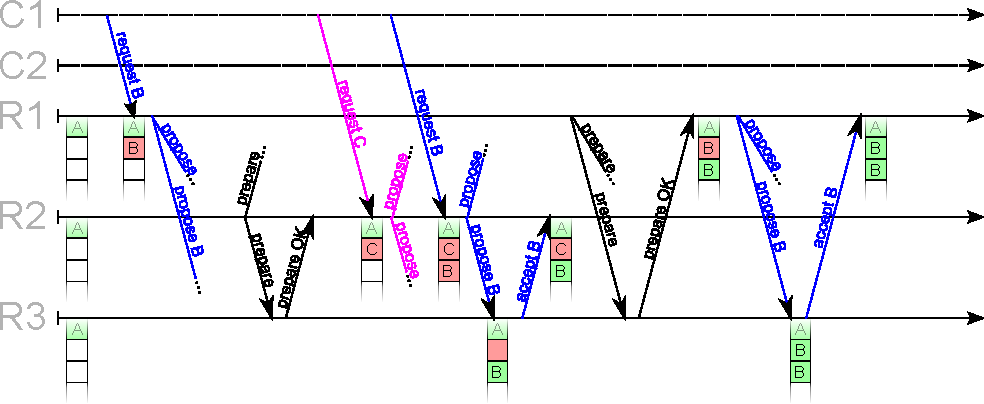
\includegraphics[keepaspectratio, width=\textwidth]{paxos/duplicating_messages.pdf}
  \caption{Duplicating messages -- the example scenario}
\end{figure}
\begin{description}
  \item[Scenario] There are three replicas - $R_1$, $R_2$ and $R_3$. $R_1$ is the leader, proposes <1:B> (value B in first consensus instance). No other processes receives these messages and $R_2$ becomes the leader. $R_2$ proposes <1:C> and <2:B>. All proposes for <1:C> are lost, but <2:B> is decided. $R_2$ fails and $R_1$ becomes the leader again. While preparing, it learns about <2:B>. It has <1:B> as a previously accepted value. The Paxos algorithm requires $R_1$ to propose <1:B> again, since its the accepted value with the highest timestamp. And this will result in the request being decided twice.
\end{description}

Unfortunately we cannot prevent requests from being decided twice in two different instances. Because of that, the only valid solution for this problem is to remember the last executed instance for every client and not executing it again. But this requires to keep a new structure in memory as well as by every snapshot (after recovering from the snapshot, this structure has to be loaded too).

Even if we cannot prevent from deciding a request twice, we should minimise the number of such situations because they slow down the algorithm (we have to send redundant data in each message). Possible solutions to decrease the scale of this problem are listed below:
\begin{itemize}
  \item We can cache the last reply for each client, so after receiving the same request we can immediately response.
  \item Do not propose requests which have been already decided
  \item The current leader can save which requests were proposed by him (but not decided yet) and also discard them.
\end{itemize}

\paragraph{Setting the window size}
The windows size specifies how many concurrent instances can be started (it has very similar meaning to the window size in the TCP protocol). In order to use available resources and keep high responsiveness the window size must be set correctly. There is no global, generic solution: every usage needs different setting.

The most important thing is monitoring the network: its usage should be high, but no congestion should occur.
That means, on one side, the window size must be enlarged as long as the links are not full, and on the other side, it must be guaranteed that no message will be delayed or dropped because of the network traffic. As long as the two conditions hold, a speed of a single instance remains constant (putting aside CPU time).
If network is overused, the overall throughput may even stay on the same level, but the latency will increase for sure.

If the instances would be decided out of order the JPaxos performance would not be affected much. But the state machine must get the requests in proper order, so the execution of requests with greater IDs would have to be delayed. And this causes inefficient request arrival time for the service. So the number of concurrent instances should not be increased if it does not increase the JPaxos throughput.

\paragraph{Performance gains}
A single instance will nearly never use available bandwidth, so conducting concurrent instances will surely speed up JPaxos.

As already mentioned, using the concurrent instances will improve latency and throughput. Carefulness is required in order to avoid network saturation, especially the link of the leader which has to carry $2n$ messages for each instance (as opposed to 2 messages for every other link).

In full-duplex networks, concurrent instances will improve network utilisation, because when the leader is waiting for replies, the network from the leader to the others is idle, so it can be used to send the next request. 

% TODO remove this paragraph?
\paragraph{Batching} is another method for improving performance and network usage. It is preferred over increasing the concurrent instances count, however joining these two methods is better than any of them alone. Batching is described in section \ref{sec:batching}, as it does not concern the Paxos protocol, but values passed to the Proposer.

\section{Batching}
\label{sec:batching}
Batching means using the same consensus instance to order several requests.

This optimisation does not need any changes to the Paxos algorithm, only requires that requests from one instance can be ordered deterministically by each replica, so that replicas know the order in which they should execute the requests. That is no problem, as a byte stream is already ordered -- so each replica will decode the requests the same way.

To achieve multiple requests in the same instance an additional activity must be taken up by the proposer and later, by replica, just before execution.

The proposer needs to \textit{stick} together the requests, and from that moment on they are treated as one. The other part, dividing it again into requests, should be done after the decision has been taken.
\begin{figure}[h]
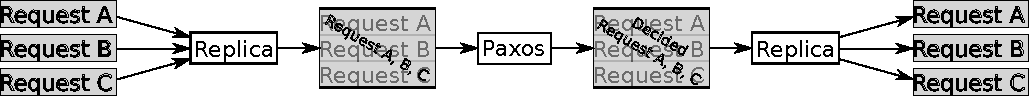
\includegraphics[keepaspectratio, width=\textwidth]{features/batching.pdf}
\vspace{-1em}
\caption{The batching mechanism}
\vspace{-1em}
\end{figure}

As the count of concurrent instances is bounded (see subsection \ref{subsec:concurrent_instances}), without batching every client needs to wait for his own instance. With batching many client requests may be \textit{packed} in one instance. That, on one side, increases the throughput and decreases the delay.
On the other side, the message size is getting bigger -- and that means slower voting.

Here arises a question: how many requests to batch? One boundary is quite obvious -- a serialized message should not be bigger than the transport protocol frame size. As for UDP the size is about 65kB, but for TCP stays unbounded.

The network bandwidth is the upper bound of peformance. Increasing the size of the instance value does not change the CPU time needed to decide on this instance. So the best performance is achieved as the batching size is set to the minimal size when all available bandwidth is used.

Another problem concerns the proposer: should there be a lower limit of requests in one instance? Doing so implies waiting for new client requests to come. Not waiting means sometimes severe throughput loss.

A new request may come a long time after we begun gathering the requests for batching -- and that would cause an unacceptable delay. So if we choose to wait for new client requests, we need to set up a timeout after which we stop waiting for the new requests and start deciding the requests we manged to gather.

If we decide not to wait at all we are packing all client requests we got until now into a single request (if it fits, of course). Such approach guarantees good behaviour if the system state is not changing. Under load  we are usually unable to pack all requests we got into single instace, while with small amount of requests no delay by packing decreases the latency.

Both the batching size and the timeout for gathering requests in a batch is configurable in our library.


\section{No operation command}

When concurrent instances optimisation is used, it is possible that leader after prepare phase will have a gap in the log. To illustrate the problem, let's analyze the scenario below.

\begin{description}
  \item [Scenario] We have three replicas $R1$, $R2$ and $R3$. Replica $R1$ is the leader and proposes <1:A> and <2:B>. Value <2:B> is decided by all replicas, but no other process receives <1:A>. $R1$ crashes and $R2$ becomes a new leader. After prepare phase, $R2$ has a gap in the log because no information about instance 1 was received.
\end{description} 

As we can see after the prepare phase, a leader can have a gap in the log. Without filling this gap, replica cannot execute and propose new values. Because of that, a new value has to be proposed in this place.

With crash-stop or crash-recovery without stable storage the value may be lost forever. That happens when decision $k+1$ is already decided, and decision $k$ is unknown to all but the leader, and the leader crashes. As only he got the value, and it has been lost -- either because he is not allowed to recover, or he is recovering without stable storage.

On the other hand, the leader change may happen due to the lost of \alive message. In this case someone has the value, and it could be used back in the voting. But there is no simple and fast method to detect this situation.

The easiest solution is to create a new request type called no-op, which is a null operation that will be ignored by the replicas. It fills the gaps but is not executed by the state machine.

\section{Log truncation}

The replicated log cannot be allowed to grow forever, it must be bounded in any practical system. After any replica executes some command, it no longer needs the corresponding log entry locally. But other replicas may not have learnt the decision yet. In this case, these late replicas need to learn the decision by asking the corresponding log entry from a replica that still has it.

In JPaxos the Paxos protocol is not used for getting lost requests due to performance reasons. For this we use a special procedure called \textit{catch-up}, which is described in section \ref{sec:catch_up}.

Having the old log is needed in three cases: for the catch-up, for view change and, in the crash-recovery model, for recovery.
The catch-up needs old log in order to send them to a replica which is not up to date, once the replica requests them.
During the view change the leader requests log entries of all instances it considers to be undecided.
By recovery a replica needs the log of other replicas in order to know what has been decided at least since its crash.

Especially the latter is problematic. The view change always requires a bounded number of instances in the log. But if we assume recovery with minimal or no stable storage (as in the case of the epoch based or view based recovery algorithm), after the recovery a replica needs to recover the state from scratch. For this, it needs the whole log or complete state.

\paragraphNewline{Global Commit Point}

A command can be deleted from the log after being executed by all replicas in crash-stop and crash-recovery models with stable storage. The highest instance executed by all replicas is called a \emph{global commit point}.

But removing all instances prior to the global commit point is not enough to ensure that the log is kept bounded, because a correct replica may be disconnected from the system for some time. When communication is reestablished, the replica needs to learn about all the decisions taken in the meantime. If one replica crashes, the other replicas have no way of knowing that it is a crash and not a disconnection, so they would have to keep the logs forever. And the replica can stay crashed for arbitrary long time.

Therefore using snapshotting is the only acceptable solution in JPaxos.

\paragraphNewline{Snapshotting}

A replica needs the old log entries in order to bring its state up to date. But instead of executing all decided requests the replica may transfer the state of the service from other replica. To transfer the state of the service some assumption must be fullfilled: the service must be able to save its state, and be able to update itself to such state.

The service can create a \textit{snapshot} -- arbitrary data that can be parsed by the service to change its state to the state identical as in the moment when the snapshot was created.

The mechanism of managing such snapshots is called by us \textit{snapshotting}.

In order to be able to remove stale log entries snapshotting must to be implemented. It also speeds up the recovery and process of filling missing instances.

The size of a snapshot is of course bounded. If we create a new snapshot as the log size reaches some limit the size of the log is bounded as well, so no structure is allowed to grow forever.

When a new snapshot is created the old log entries are truncated. If a replica that is missing old logs rejoins, the most recent snapshot is transferred first and then all the decisions since the snapshot are sent to complete the updating procedure.

The most problematic part is the Service -- if it does not implement creating snapshots or does not provide them often enough, the log will grow forever.

Snapshotting is described in details in the section \ref{sec:snapshotting}.

\section{Skipping redundant messages}
Reducing the number of messages is one of the most efficient optimisations. In JPaxos a process does not send messages to itself, also the proposer does not send \accept messages to anyone.

It has been proven for the Paxos consensus algorithm that it minimises the number of messages carrying a value to be agreed upon (the client request in our case). The value is sent only once to each replica (not counting retransmission due to message loss). As for additional messages, their count varies among certain implementations. Some of messages proposed in the typical implementation may be easily skipped without violating guarantees or adding any assumptions.

\paragraphNewline{Using {\normalfont\propose}as {\normalfont\accept}}

Another optimisation is merging the role of \accept and \textsc{Propose}. As long as acceptors and proposes do not share the log this is not allowed. But if their knowledge is identical and the leader proposed some value, then he must accept it as well. In most solutions one node acts as proposer and acceptor, and they do share the log.

So in JPaxos each \propose is simultaneously an \accept message. Notice that if the system consists of three nodes every process decides on the value by receiving a valid propose -- it knows that the leader and itself
accept the message. Normally the leader process has to first send \propose to all and later \accept to all. By this optimisation only half of messages is required to be sent.

\paragraphNewline{Sending to itself}

As stated before, Paxos defines three types of roles: proposers, acceptors and learners. Processes or some of their parts act as one of them. In order to communicate they must send messages to each other.

In our program every node consists of a (probable) proposer, acceptor as well as learner. In this case there is no need to send messages to self. Especially all send-to-all commands may be replaced by send to others command, as long as the communication with self will be done internally. This skips one \accept and one \propose sent by the leader, and one \accept by all other processes.

This does not influence performance much, however it is recommended as it decreases the use of system resources (especially the networking stack). It also skips a few system calls.

\paragraphNewline{Minimizing the count of messages carrying the value}

Most of the articles about Paxos state that the \accept message carries the value (request from client).
In such case we can accept on the value even without receiving a \propose message.

The value usually is bigger than a normal message of JPaxos. Because of that we want to minimize number of messages which contain the value.
In JPaxos the \accept message does not carry the value. Before a process can send the \accept message it has to receive the \propose message. The process decides upon a value if it receives a \propose and majority of \accept messages.

Waiting for the \propose message might cause additional overhead, but usually the \propose will be delivered prior to the majority of \accept messages.
Each process must receive one \propose[], but multiple \accept messages. If the \accept message does not carry the value, significantly less network bandwidth is used by a single instance.


\paragraphNewline{Best-case messages}
\label{par:bestCaseMessages}
So, in the normal operation in JPaxos:

%TODO: TZ: Jeśli masz sprawnego inkscape'a, narysuj proszę do tego prosty rysunek best case 
% mi nie tylko vim'a popsuł niedokończony update systemu, inkscape też narzeka na brak jakiegoś .so
% chodzi o diagram odpowiadający komunikacjom z tabelki poniżej
\begin{figure}[ht]
  \centering
  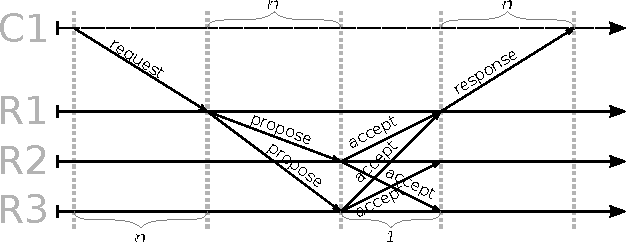
\includegraphics[keepaspectratio, width=0.8\textwidth]{best_case.pdf}
  \caption{Best-case scenario}
\end{figure}

\begin{table}[h]
\begin{tabular}{rccccc}
          & \begin{tabular}{c} How many \\ processes send \\ the message \end{tabular} 
          & \begin{tabular}{c} Count of \\ messages \\ sent \end{tabular} 
          & Time 
          & \begin{tabular}{c} Message \\ type \end{tabular}
          & \begin{tabular}{c} Carries value \\ (client requests) \end{tabular}
          \\
 Proposer & $1$                     & $n-1$             & $n$  & \propose & yes    \\
 Acceptor & $n-1$                   & $n-1$             & 1    & \accept  & no
\end{tabular}
\end{table}

We can see that in order to decide the process needs to send the \propose[] once, and later each non-leader process sends the \accept to others.

For the comparison of consensus algorithms usually time is defined in a specific way: $n$ denotes the time needed to send a message containing the value to be agreed upon, and $1$ is the time required to send any other message. This is motivated by the value size -- usually the value is significantly bigger than any protocol message, so it is important to differentiate the messages carrying value and all the others.

Other implementations consider using bounded learner count -- only some processes are selected as the learners. For example only one process plays the role of a learner -- that means the acceptors send the \accept messages only to this process. An additional message, \textsc{Decided}, is sent by the learner to all as the ballot has finished. Thanks to this modification no reliable broadcast is needed, but also an additional phase of communication must occur. If only some processes act as learners, it is important to ensure that there is at least one learner that didn't crash, otherwise the protocol would not guarantee liveness.

An interesting approach is presented in the RingPaxos (see \cite{Mar10}), where IP-multicast is used for all broadcasts, what significantly increases the scalability and performance.

\chapter{Recovery}
\label{chapter:recovery}

In this chapter we describe the recovery of process from crash. We present 3 different algorithms implemented in JPaxos with different performance and fault tolerance. We will start from short overview of recovery and then present 4 different algorithms -- crash-stop, crash-recovery with stable storage, epoch based recovery and view based recovery. After that we will summarize and compare all algorithms.

\section{Overview}

The crash of the process is a permanent lack of activity from a program. It may be caused by programming error, lack of electricity etc. Such process also losses all information not saved to stable storage.

So what is stable storage? The process can write data to different places, it can be processor cache, RAM, hard drives, etc. We can divide them into two categories - the one where data can survive the crash, and the other where data is lost after a crash. All memory holders from first category will be called stable storage and from second category volatile storage.

Usually operating system buffers the data before writing it to stable storages. Such writes are called asynchronous. They do not provide guarantee that if crash occurs, all data will be on the storage instead of being lost with the rest of system buffer.

Another option is to force the operating system to write the data to stable storage. Such operating is called \emph{synchronising} the buffers with storage. If we call write and synchronise, we can say that the write is synchronous -- the data won't be lost due to crash. But writing to stable storage synchronously is very slow, so we want to minimize the amount of writes on critical path.

In following sections, we will use below variables: 
\begin{tightList}
  \item[$n$] -- number of processes
  \item[$f$] -- number of faulty process
  \item[$p$] -- the id of local process
\end{tightList}

\section{Crash stop}
\label{sec:crash_stop}

Let's start from the easiest scenario -- the crash-stop model. In this model crashed process will never be up again.
Because of that there is no recovery phase and we don't need a stable storage. Because process does not do any synchronous writes to stable storage the performance is very high. 

But there is one big drawback. In previous chapters we said that Paxos algorithm can decide on the value (can continue working) if majority of processes are correct. If majority of processes will crash in this model, the algorithm will never decide again and our replicated service will stop forever. Because of that using this model is not very practical. Below we present 3 algorithms which allow for process recovering.

For performance tests and for theoretical purposes this model is very important -- it is the fastest model, used as comparison point with others. It is easier also to analyze correctness of this model and prove that the algorithms implementing recovery models are correct taking under consideration only the changes in the code.

\section{Recovery phase}

A recovery phase is the state of JPaxos replica after starting the process. It must be decided, if this is the first run of this replica or recovery from crash.

Of course, if this is the first start, the process can just go to normal state. Otherwise the process must stay in the Recovery phase as long as it does not fulfill requirements of the recovery model.

The process cannot join the Paxos protocol until the recovery phase is finished. So recovering process cannot respond to any message received, like \propose[], \accept[], \prepare and \prepareOK[]. However, these messages may be received and processed, so the process can passively join the protocol. The moment when the process joins (actively) Paxos protocol is also a moment when the process is considered as correct.


\section{Crash-recovery with stable storage}
\label{sec:full_ss}

First algorithm with ability to recover a process is crash recovery with stable storage. In this algorithm, we want to save all necessary data to stable storage. After crash the process can load all information from stable storage and join the Paxos protocol. To increase the performance the process should write as little as possible and as rare as possible to stable storage.

Description of variables used in algorithm below:
\begin{tightList}[\setlength{\labelwidth}{20em} \setlength{\leftmargin}{2\leftmargin}]
  \item[$log_p$] -- the array of consecutive instances -- $id \rightarrow <view, value>$
  \item[$view_p$] -- the current view number
  \item[$state_p$] -- the last snapshot made by service or received from catch-up
\end{tightList}

\begin{algorithmic}[1]
  \INIT{}
    \STATE $log_p \leftarrow \bot$ %\COMMENT {In-memory log}
    \STATE $view_p \leftarrow 0$
    \IF{$view_p \mod n = p$}
      \STATE $view_p \leftarrow 1$
    \ENDIF
    \STATE $state_p \leftarrow \bot$ %\COMMENT{The last snapshot}
    \STATE
    \IF{recovery after crash}
      \STATE $view_p \leftarrow$ last view number written to stable storage
      \FOR{$<id, view, value>$ from stable storage}
        \STATE $log_p[id] \leftarrow <view, value>$
      \ENDFOR
      \STATE $state_p \leftarrow$ last snapshot saved to stable storage
    \ENDIF
    \STATE
    \STATE join Paxos protocol
  \ENDINIT

  \vspace{1em}
  \PROCEDURE{advanceView(view)}
    \STATE write $view$ to stable storage
    \STATE $view_p \leftarrow view$
  \ENDPROC

  \vspace{1em}
  \PROCEDURE{updateValue(id, view, value)}
    \STATE $log_p[id] \leftarrow <view, value>$
    \STATE write $<id, view, value>$ to stable storage
  \ENDPROC

  \vspace{1em}
  \PROCEDURE{newSnapshot(snapshot)}
    \STATE write $snapshot$ to stable storage
    \STATE $state_p \leftarrow snapshot$ 
  \ENDPROC
\end{algorithmic}

On recovery the algorithm reads the view, values for all consensus instances and last snapshot from stable storage and can join a Paxos protocol (the process cannot respond to any message until it loads everything from stable storage).

This synchronous writes are made on critical path, so the performance of this algorithm will be much lower comparing to crash-stop model. But the crash recovery with stable storage algorithm tolerates catastrophic failures -- the failure when all processes crashed. Of course when the majority of the processes will be crashed, the replicated service will be unavailable. But we can start all processes again and they will recover to state from before the crash.

As we can see, this algorithm is already deployable in environment with crashes. But because the performance is really low, we will introduce two more algorithms. These algorithms will not tolerate catastrophic failures but their performance should be close to performance of crash-stop model.

\section{Epoch based recovery}
\label{sec:epoch_ss}

In this section, we will describe the algorithm based on epoch numbers. This algorithm is making only one synchronous write to stable storage on process startup, but the recovery phase is more complicated comparing to previous algorithm.

We will use following variables in the pseudocode:
\begin{tightList}[\setlength{\labelwidth}{20em} \setlength{\leftmargin}{3\leftmargin}]
  \item[$epoch_p$] -- vector of epoch numbers
  \item[$e$] -- epoch number of single process
  \item[$highestId$] -- the id of highest known consensus instance
\end{tightList}

The pseudocode below should explain this algorithm:
\begin{algorithmic}[1]
  \INIT{}
    \STATE $log_p \leftarrow \bot$ %\COMMENT {In-memory log}
    \STATE $view_p \leftarrow 0$
    \IF{$view_p \mod n = p$}
      \STATE $view_p \leftarrow view_p + 1$
    \ENDIF
    \STATE $state_p \leftarrow \bot$ %\COMMENT{The last snapshot}
    \STATE $\forall q : epoch_p[q] \leftarrow 0$
    \STATE
    \IF{recovery after crash}
      \STATE $epoch_p[p] \leftarrow$ last epoch number written to stable storage
      \STATE $epoch_p[p] \leftarrow epoch_p[p] + 1$
      \STATE send $<\recovery, epoch_p[p]>$ to all except $p$
      \STATE wait for $n-f <\recoveryAnswer, epoch, view, highestId>$ messages including from primary of highest view received
      \STATE $\forall s \in \Pi : epoch_p[s] \leftarrow \max\{{epoch[s] \; \mathrm{ received}}\}$
      \STATE $view_p \leftarrow \max\{{ view \; \mathrm{received}}\}$
      \STATE download all instance up to $highestId$ from leader using catch-up module
    \ENDIF
      \STATE write $epoch_p[p]$ to stable storage
    \STATE
    \STATE join Paxos protocol
  \ENDINIT

  \vspace{1em}
  \UPON{receive $<\recovery, e>$ from $q$}
    \IF{$q$ is primary of $view_p$}
      \STATE change to a higher view where $q$ is not primary
      \STATE wait until view change is complete
    \ENDIF
    \STATE $epoch_p[q] \leftarrow e$
    \STATE send $<\recoveryAnswer, epoch_p, view_p, highestId_p>$ to $q$
  \ENDUPON

  \vspace{1em}
  \UPON{$<\prepareOK, epoch, view, highestId>$ from $q$}
    \IF{$view > view_p$}
      \STATE $view_p \leftarrow view$
      \STATE send $<\prepare, view_p>$ to all
    \ELSE
      \STATE $\forall q : epoch_p[q] \leftarrow \max\{{epoch[q], epoch_q[q]}\}$
      \FORALL{$s \in \Pi$}
        \STATE discard all messages $<\prepareOK, epoch, view_p, -, ->$ from $s$ where $epoch[s] < epoch_q[p]$
      \ENDFOR
      \STATE execute normal handler 
    \ENDIF
  \ENDUPON
\end{algorithmic}

Epoch based recovery algorithms tolerates $f = \left\lfloor \frac{n-1}{2} \right\rfloor $ crashed processes. It is required that at least majority of processes are always correct - otherwise the algorithm will not be able to continue.

In recovery phase the process first notifies the majority of other replicas about it's recovery. As the process must know when it's state will be correct, it must wait for recovery answer from the leader, who has the most recent state. Once it gets the acknowledges, it is downloading all information from other replicas using catch-up mechanism.  When all necessary information is transfered, the replica can join the Paxos protocol and is considered as correct.

On normal execution this algorithm should be as fast as crash-stop model. The size of \prepareOK message is increased by epoch vector which contains $n$ numbers but it shouldn't have big impact on performance or network usage. This algorithm is a compromise between crash-stop and crash-recovery with stable storage.  

\subsection{Example}

Let's analyze one example to better understand this algorithm. Assume that we replicate service on $n = 5$ replicas. All processes are numbered from 0 to 4, have initial epoch vector $[0, 0, 0, 0, 0]$, are initially correct and are in view 4 (where process 4 is a leader).

Process 0 is suspecting a leader and changing view to 5 by sending \prepare message to all. Process 1 receives \prepare and respond with $<$\prepareOK[], [0, 0, 0, 0, 0], 5, -$>$. The process 0 receives the response and process 1 crashes. After crash process 1 is recovering, increases epoch number to 1 and sends $<$\recovery[], 1$>$ message to all. Processes [2, 3, 4] receives \recovery message, updates epoch vector to [0, 1, 0, 0, 0] and responds with \recoveryAnswer and view 4. After receiving three \recoveryAnswer messages with view 4 (also from leader of view 4), process 1 joins the protocol with view 4. Now process 2 receives the \prepare from process 0 and responds with $<$\prepareOK[], [0, 1, 0, 0, 0], 5, -$>$.

Process 0 already received 3 \prepareOK responses, from [0, 1, 2]. But message from process 1 will be discarded because it was sent when process 1 was in epoch 0 and now from process 2 we know that process 1 is in epoch 1. If we wouldn't discard this message, process 0 would be prepared leader in view 5 but processes [1, 3, 4] would be in view 4 and that would cause violation of Paxos protocol.

\begin{figure}[h]
 \centering
 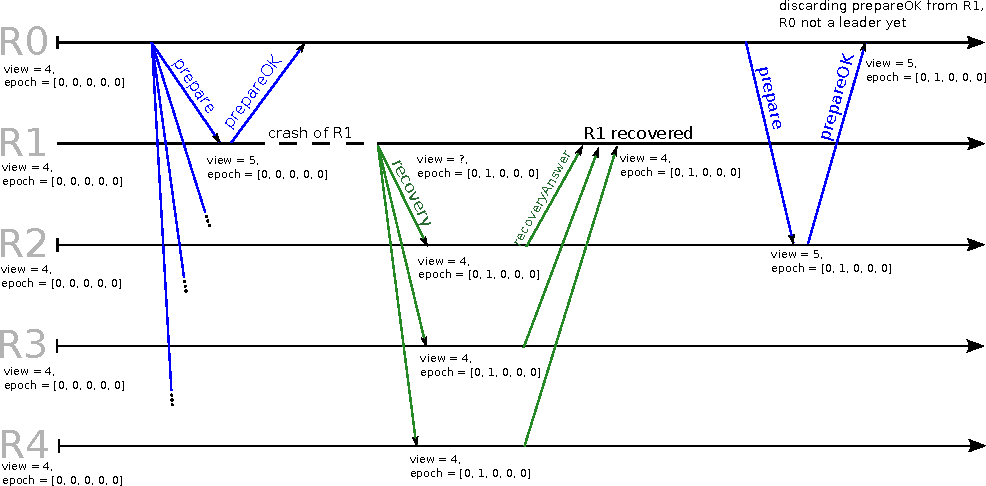
\includegraphics[keepaspectratio, width=0.9\textwidth]{epoch_recovery.pdf}
 \caption{Example of epoch based recovery}
 \label{fig:epoch_based_recovery}
\end{figure}

\section{View based recovery}
\label{sec:view_ss}

The next algorithm is view based recovery. It has similar properties to epoch based recovery. In every moment majority of processes is required to be correct but instead of using epoch numbers, the view number is written to table storage on every change. 

The pseudocode of this algorithm is presented below: 

\begin{algorithmic}[1]
  \INIT{}
    \STATE $log_p \leftarrow \bot$
    \STATE $view_p \leftarrow 0$
    \IF{$view_p \mod n = p$}
      \STATE $view_p \leftarrow view_p + 1$
    \ENDIF
    \STATE $state_p \leftarrow \bot$
    \STATE
    \IF{recovery after crash}
      \STATE $view_p \leftarrow$ last view number written to stable storage
      \IF{$view_p \mod n = p$}
        \STATE $view_p \leftarrow view_p + 1$
      \ENDIF
      \STATE send $<\recovery[], view_p>$ to all except $p$
      \STATE wait for $n-f <\recoveryAnswer[], view, highestId>$ messages including from primary of highest view received
      \STATE $view_p \leftarrow \max\{{ view \; \mathrm{received}}\}$
      \STATE download all instance up to $highestId$ from leader using catch-up module
    \ENDIF
    \STATE
    \STATE join Paxos protocol
  \ENDINIT

  \vspace{1em}
  \PROCEDURE{advanceView($view$)}
    \STATE write $view$ to stable storage
    \STATE $view_p \leftarrow view$
  \ENDPROC

  \vspace{1em}
  \UPON{receive $<\recovery[], view>$ from $q$}
    \IF{$q$ is primary of $view_p$}
      \STATE change to a higher view where $q$ is not primary
      \STATE wait until view change is complete
    \ENDIF
    \IF{$view > view_p$}
      \STATE advanceView(view)
    \ENDIF
    \STATE send $<\recoveryAnswer[], view_p, highestId_p>$ to $q$
  \ENDUPON
\end{algorithmic}

This algorithm makes synchronous write to stable storage on every view change. If the network is stable and the leader doesn't crash, performance of the algorithm should be the same as in crash-stop model. If the view is change often because of message loss or leader crash, the performance can decrease.

The recovery phase is quite similar to the epoch based recovery. Recovering process is sending \recovery message to all and waits for majority of \recoveryAnswer to get $heighestId$ value from leader. Then catch-up mechanism is used to retrieve missing instances from correct processes. This algorithm is easier than based on epoch, because it doesn't introduce any changes in handling \prepareOK message.

\section{Comparison}

We presented 4 different algorithms implemented to JPaxos library. Each algorithm has different performance and fault tolerance. To choose the best algorithm for user service, we need to decide what fault tolerance and performance is required. In the table below we present the comparison of all algorithms by comparing:
\begin{table}[h]
  \footnotesize
  \begin{tabular}{lccccc}
                        & Crash-stop & Full stable storage & View based      & Epoch based \vspace{0.2em} \\
    Decides by          & $2f+1$     & $2f+1$              & $2f+1$          & $2f+1$      \\
    Fault tolerance     & $2f+1$     & $f$                 & $2f+1$          & $2f+1$      \\
    Process can recover & no         & yes                 & yes             & yes         \\
    Stable storage use  & no         & per round           & per view change & on recovery \\
    Additional messages & ---        & ---                 & \recovery       & \recovery   \\
    State transfer      & no         & if needed           & yes             & yes         \\
    Increased msg size  & ---        & ---                 & ---             & \prepareOK by $n$\\
  \end{tabular}
  \caption{Comparison of recovery algorithms.}
  \scriptsize
\end{table}

\begin{figure}[h]
 \centering
 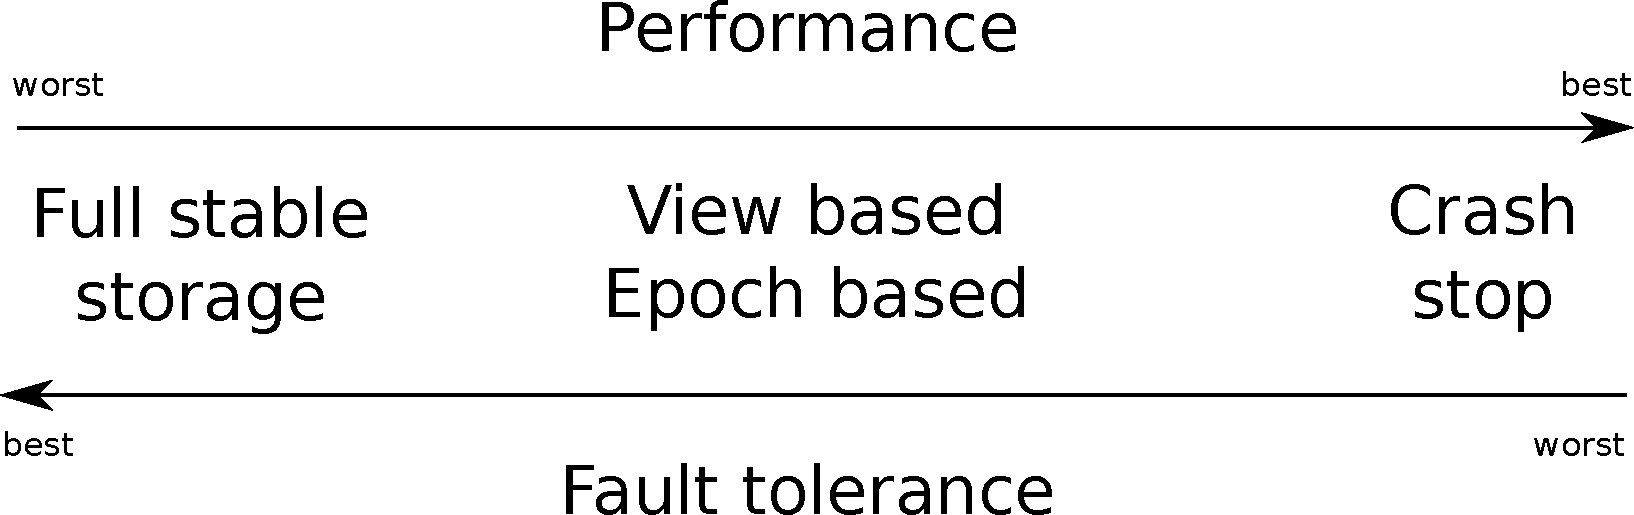
\includegraphics[keepaspectratio, width=0.75\textwidth]{recovery_algorithms.pdf}
 \caption{Comparison of recovery algorithms}
 \label{fig:recovery_algorithms}
\end{figure}

Crash recovery with full stable storage is an algorithm with the best fault tolerance because it tolerates catastrophic failures. But to achieve that it makes a synchronous writes to stable storage on every round (on every view and value change) what decreases the performance.

Crash stop doesn't provide any recovery (crashed processes will never be correct again) and all the time majority of processes have to be correct. But no synchronous writes to stable storage are made so it provides the best performance.

The compromise between crash recovery with stable storage and crash stop are view based and epoch based recovery. They support recovery of crashed process and their performance should be close to crash-stop model. If service doesn't have to tolerate catastrophic failures, it is the best to use them in production environment.

Proofs of all algorithms presented in this chapter can be found in \cite{Nun10}. 

\chapter{Conclusions}

In this thesis, we have studied the problem of state machine replication based
on the Paxos algorithm defined in \cite{Lam98}. We described challenges faced in
the implementation phase to make the library ready to use in production systems,
with support of crash-recovery model, message loss and communication delays.

We first presented the Paxos algorithm with theoretical background. Then we
focused on the problems that occur when a single page of distributed algorithm
pseudocode is transformed to ten thousand lines of production code. We
presented the architecture of our library, with short description of every
module and data structure used. The library has to handle unreliable network
with message loss and delays, so we presented the catch-up mechanism, which
guarantees that eventually every correct replica will be up to date. By
introducing snapshot mechanism, we solve the problem of keeping the log size
bounded. To improve the efficiency of JPaxos, we implemented several
performance improvements like concurrent instances, skipping redundant messages
and batching. To tolerate crash-recovery model, four different recovery
algorithms have been implemented and described in this paper.

To test the library we implemented replicated hash map as an example of
deterministic service. We used it to verify that our library is working
correctly and that API we provide is user friendly. Our library is used as 
communication layer in PaxosSTM master thesis \cite{Tad10}.

Our future work includes introducing further performance improvements to JPaxos
and adding support for crash-recovery models without the stable storage at all.
It~would be also interesting to evaluate all recovery algorithms in a network
with message loss and environment when failure of replica is a common scenario.
Finally, we would like to publish the library as open source project and test
it in production environment.

\section*{Acknowledgments}

The work described in chapters 3, 4 and 5 was partially done by the authors during
their internship at École Polytechnique Fédérale de Lausanne (EPFL) in July and
August 2009, under supervision of dr Nuno Santos and prof.\ Andre Schiper. We
thank prof.\ Schiper for mentoring us during our stay at EPFL. We thank Nuno for
initial implementation of JPaxos, discussion about design of JPaxos, for making
benchmarks, for presenting recovery algorithms and for help with implementation
issues.

This work has been partially supported by the Polish Ministry of Science and
Higher Education within the European Regional Development Fund, Grant No.\
POIG.01\-.03\-.01-00-008/08. The two months stay at EPFL during the summer of 2009
was supported by EPFL within the Summer@EPFL internship program.

We would like to thank Tadeusz Kobus and Maciej Kokociński from Poznań University
of Technology, the developers of PaxosSTM, for testing our library and
discussion about JPaxos API.

\cleardoublepage


% All appendices and extra material, if you have any.
\cleardoublepage\appendix%
\newcounter{pageTemp}
\setcounter{pageTemp}{\value{page}}
\pagenumbering{roman}
\chapter{JPaxos user guide}

\section{Overview}
\label{overview:overview}\label{overview::doc}\label{overview:jpaxos-user-guide}
JPaxos is a Java library and runtime system for efficient state machine
replication. With JPaxos it is very easy to make a user-provided
service tolerant to machine crashes. Our system supports the \emph{crash-recovery}
model of failure and tolerates message loss and communication delays.
\begin{description}
\index{State machine replication}\item[{\href{http://en.wikipedia.org/wiki/State\_machine\_replication}{State machine replication}}] \leavevmode\phantomsection\label{overview:term-state-machine-replication}
is a general method for implementing a fault-tolerant service by
replicating it on separate machines and coordinating client interactions
with these replicas (or copies). The physical isolation of machines in
a distributed system ensures that failures of server replicas are
independent, as required. As long as there are enough of non-faulty
replicas, the service is guaranteed to be provided.

\end{description}

JPaxos makes the following assumptions about the replicated service:
\begin{itemize}
\item {} 
deterministic behaviour, i.e. multiple copies of the service begun in
the start state, receiving the same inputs in the same order will
arrive at the same state having generated the same outputs

\item {} 
non-Byzantine failures, i.e. a service machine can only crash

\item {} 
crash-recovery supported, i.e. after crash, the service can be restarted
with the same IP address.

\end{itemize}


\subsection{Two execution modes}
\label{overview:two-execution-modes}
JPaxos can be run in one of the following two modes of operation
(the mode is set up from the configuration file at system start up
and cannot be changed at runtime):

Basic mode
\begin{itemize}
\item {} 
to be able to tolerate $f$ faulty replicas, the system must consists
of at least $2f + 1$ replicas (i.e. $n \ge 2f + 1$)

\item {} 
after replica crash, it recovers its state from other replicas

\end{itemize}

Extended mode
\begin{itemize}
\item {} 
no limit on the number of faulty processes (i.e. $f = n$)

\item {} 
after replica crash, it recovers its state from non-volatile memory

\item {} 
around 200 times slower than the basic mode

\end{itemize}


\subsection{Simple API}
\label{overview:simple-api}
For the end user JPaxos provides:
\begin{enumerate}
\item {} 
\code{Service} interface -- it specifies a few methods for interfacing
the user-defined servi\-ce code with JPaxos; our library provides
abstract classes implementing \code{Ser\-vice} interface, making it easier to
to create a new service (state machine);
see {\hyperref[api:jpaxos-service]{\emph{Service interface}}} for details

\item {} 
\code{Replica} class -- that should be instantiated and started
(see {\hyperref[api:jpaxos-replica]{\emph{Replica}}} for details)

\item {} 
\code{Client} class -- the part that may send request to be executed
(see {\hyperref[api:jpaxos-client]{\emph{Client}}} for details)

\end{enumerate}

The \code{Service} and \code{Replica} are bound to each other, while
\code{Client} can be located anywhere.

JPaxos guarantees that in crash-recovery model, with static groups,
lossy network with any delays:
\begin{itemize}
\item {} 
if the client sends a request, it'll eventually get the answer

\item {} 
every replica will execute the request exactly once

\item {} 
any two replicas will execute the requests in the same order

\end{itemize}


\subsection{Distributed implementation}
\label{overview:distributed-implementation}
JPaxos is a fully distributed implementation, which means that there
is no predefined central coordinator that might be a bottle-neck or a single
point of failure in the system.

For this, JPaxos implements
the \href{http://en.wikipedia.org/wiki/Paxos\_algorithm}{Paxos}
distributed algorithm with various optimizations, in order to efficiently
deliver client requests to all service replicas despite any failures.
Replicas receive all requests globally ordered, thanks to
the total-order (or atomic) broadcast protocol implemented on top
of Paxos.

Figure below shows processing of a single request message submitted
by the Client to the replicated state machine:
\begin{quote}
\begin{figure}[htbp]
\centering

\scalebox{0.500000}{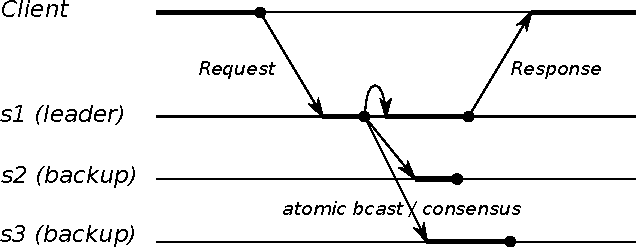
\includegraphics{user_guide/state_machine.pdf}}
\end{figure}
\end{quote}

where \emph{Client} is an instance of the \code{Client} class, while \emph{s1}, \emph{s2},
and \emph{s3} are instances of the \code{Replica} class.

If a request is delayed or lost due to the network or replica failure,
after a timeout, it will be reissued by the \emph{Client}, as illustrated in
Figure below:
\begin{quote}
\begin{figure}[htbp]
\centering

\scalebox{0.500000}{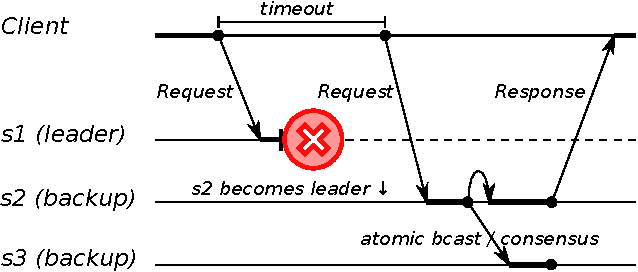
\includegraphics{user_guide/state_machine_crash.pdf}}
\end{figure}
\end{quote}


\section{Deployment and configuration}
\label{config:deployment-and-configuration}\label{config::doc}
This section presents quick overview on what is necessary to compile the
library and how to configure the system and start the example which is included
in the distribution.


\subsection{Deployment requirements}
\label{config:deployment-requirements}
JPaxos requires the following components to be installed on the target system:
\begin{itemize}
\item {} 
\href{http://www.java.com/}{Java JRE 1.5} or later

\end{itemize}

Additionally, the following are optional but helpful tools in compilation and
packaging:
\begin{itemize}
\item {} 
\href{http://ant.apache.org/}{Apache Ant} -- used to run all build scripts (distributed under the Apache
License 2.0)

\end{itemize}


\subsection{Configuration file}
\label{config:configuration-file}
The format of configuration file used by \code{Configuration} class is the same as
default Java Properties file. As mentioned earlier, this file contains
nodes configuration and replica related options.


\paragraphNewline{Node configuration}
\label{config:node-configuration}
A node is configured with a single line containing \code{hostname}, \code{replica
port} and \code{cli\-ent port}, separated with commas:

\begin{Verbatim}[commandchars=@\[\]]
process.@textless[]id@textgreater[] = @textless[]hostname@textgreater[]:@textless[]replica@_port@textgreater[]:@textless[]client@_port@textgreater[]

process.0 = localhost:2000:3000
process.1 = localhost:2001:3001
process.2 = localhost:2002:3002
\end{Verbatim}

Above configuration creates three replicas with ids: 0, 1, 2. Replica with id 0,
is running on localhost and is using port 2000 to communicate with other replicas
and is using port 3000 to accept connections from clients.


\paragraphNewline{Crash model selection}
\label{config:crash-model-selection}
One should select the crash model of the system. If the crash model uses the
non-volatile memory (i.e. hard drive), the location of the logs may be
specified as well.

Currently supported crash models include:

\begin{tabular}{|L|L|L|L|}
\hline
\textbf{
Type
} & \textbf{
Name
} & \textbf{
Needs stable storage
} & \textbf{
Fault tolerance
}\\
\hline

CrashStop
 & 
CrashStop
 & 
No
 & 
minority
\\

CrashRecovery
 & 
FullStableStorage
 & 
Yes, heavy usage
 & 
catastrophic
\\

CrashRecovery
 & 
ViewSS
 & 
Yes, periodically
 & 
minority
\\

CrashRecovery
 & 
EpochSS
 & 
Yes, one write by start
 & 
minority
\\
\hline
\end{tabular}

\begin{description}
\item[{Crash model types:}] \leavevmode\begin{itemize}
\item {} 
CrashStop - once the replica crashed, it cannot recover

\item {} 
CrashRecovery - the replica may crash and subsequently recover

\end{itemize}

\end{description}

Fault tolerance ranks:
\begin{itemize}
\item {} 
minority - the minority of replicas may crash; $f = \left\lfloor (n-1)/2 \right\rfloor$

\item {} 
catastrophic - all replicas may crash; $f=n$

\end{itemize}

To select a crash model, one must add to the configuration file a line
\code{CrashModel = {[}crash model name{]}}. If no crash model is provided, the
\code{FullStableStorage} is assumed.

For choosing a log path one needs to add another line with syntax \code{LogPath =
{[}path{]}}. The logs will be actually stored in subdirectory named after replica
id in the given location. The default value for log path is \code{jpaxosLogs}.

An example configuration:

\begin{Verbatim}[commandchars=@\[\]]
CrashModel = ViewSS
LogPath = /mnt/shared/jpaxos/logs
\end{Verbatim}


\paragraphNewline{Replica options}
\label{config:replica-options}
Configuration file also allows to set additional options for replicas.
Understanding how each option described below can affect JPaxos is important to
achieve high performance.


\paragraphNewline{Window size}
\label{config:window-size}
The window size determines the maximum number of concurrently proposed
instances. The meaning of this option is very similar to window size in TCP
protocol.

To illustrate it, assume that window size is set to 10. It allows to run
instances with id's from 1 to 10 concurrently and to decide instances 2 - 10
before instance 1. JPaxos cannot execute any instance until all previous
instances are executed so because instance 1 is not decided / executed, no
instance can be executed on state machine. When instances 1 will be
decided and executed all consecutive instances will also be executed.

The example above shows that by increasing the value of window size we can
decrease the response time - a lot of instances will be decided, but none can
be executed. Because of that it is recommended to set this option to lower
value and BatchSize to higher value so that decided instances can be executed
faster.

The default value of this option is 2 and can be set using:
\begin{Verbatim}
WindowSize = 4
\end{Verbatim}

\paragraphNewline{Batch size}
\label{config:batch-size}
JPaxos will try to batch requests into a single proposal to improve the
performance. This option controls the maximum size (in bytes) of requests
grouped into one consensus instance.

For example, if maximum batch size is set to 1000 and JPaxos received requests
of size 100, 300, 400, 300 bytes, then first three requests will be batched
into one consensus instance of size 100 + 300 + 400 = 800 (the size of all four
requests is 1100 what is greater than maximum allowed batch size).

The default value of this options is 65507 bytes and can be changed by adding:
\begin{Verbatim}
BatchSize = 65507
\end{Verbatim}


\paragraphNewline{Maximum batch delay}
\label{config:maximum-batch-delay}
This option determines how long JPaxos will wait for new requests to be packed
into single instance.

The default value of this option is 10 ms and can be change using:
\begin{Verbatim}
MaxBatchDelay = 20
\end{Verbatim}


\paragraphNewline{Network protocol}
\label{config:network-protocol}
It is also possible to choose protocol used to communicate between replicas.
One may choose:
\begin{itemize}
\item {} 
TCP (default)

\item {} 
UDP

\item {} 
Generic - Uses UDP for small messages and TCP for larger messages

\end{itemize}

It is important to note that UDP protocol has message size restriction -
messages must be smaller than the maximum allowed size of UDP packet (64KB or
less, depending on the network). User must be careful with the size of client
requests and of BatchSize so that this limit is not violated. Because of this
limitations, user should choose TCP or Generic option.

If one chooses Generic, it is also recommended to set what is a `small' and
what is a `big' message, by setting maximum allowed UDP packet size:

\begin{Verbatim}[commandchars=\\\{\}]
\PYG{n}{Network} \PYG{o}{=} \PYG{n}{Generic}
\PYG{n}{MaxUDPPacketSize} \PYG{o}{=} \PYG{l+m+mi}{1000}
\end{Verbatim}

In example above, all messages smaller than 1000 bytes will be sent using UDP
and all others using TCP protocol.

\paragraphNewline{Example file}
\label{config:example-file}

Below is an example configuration file:

\begin{Verbatim}[commandchars=@\[\]]
@# Nodes configuration
process.0 = 192.168.1.5:2000:3000
process.1 = 192.168.1.6:2001:3001
process.2 = 192.168.1.7:2002:3002

@# Crash model configuration
CrashModel = EpochSS
LogPath = jpaxos/stableStorage

@# Batching configuration
WindowSize = 2
BatchSize = 65507
MaxBatchDelay = 10

@# Network configuration
Network = TCP
\end{Verbatim}


\subsection{Configuration classes}
\label{config:configuration-classes}
The user of JPaxos has to configure the system by creating instance of
\code{Configuration} class. Instance of this class is required to create the
\code{Replica} and \code{Client} (see {\hyperref[api:jpaxos-api]{\emph{Application programming interface}}} chapter).

The \code{Configuration} class either loads the setting from certain file, or the
settings may be provided by instantiating.

\code{Configuration} contains nodes configuration (information about replicas - ids,
hostnames and ports), and replica related options (batching size, window size,
etc.). \code{Client} is using only nodes configuration (hostnames and ports) and
ignores replica related options, while \code{Replica} is using all options from
\code{Configuration}.

The user is responsible for providing correct configuration to replicas and
clients. The configuration must be the same in every replica and client or else
the system may fail.


\paragraphNewline{\texttt{Configuration} class}
\label{config:jpaxos-configclass}\label{config:configuration-class}
The \code{Configuration} has three constructors available:
\begin{itemize}
\item {} 
\code{Configuration ()}
Default constructor, loads configuration from \code{paxos.pro\-per\-ties} file
located in current working directory. The structure of configuration file is
described in ``Configuration file format'' section.

\item {} 
\code{Configuration (String fileName)}
Loads configuration from file specified as constructor argument. The format
of the file is described in ``Configuration file format'' section.

\item {} 
\code{Configuration (List\textless{}PID\textgreater{} processess)}
Loads configuration using only no\-des configuration. The \code{PID} structure is
described below. Replica related options are set to default.

\end{itemize}


\paragraphNewline{\texttt{PID} class}
\label{config:pid-class}
Stores node configuration data (information about one replica):
\begin{itemize}
\item {} 
\code{id}
The id of replica. Ids start from 0.

\item {} 
\code{hostname}
The replica ip address (e.g. ``127.0.0.1'') or host name (e.g. ``localhost'').
The replicas (and clients) will use this address to establish connection with
this replica.

\item {} 
\code{replicaPort}
The port used by replicas to establish connection with this replica.

\item {} 
\code{clientPort}
The port used by clients to establish connection with this replica.

\end{itemize}


\section{Application programming interface}
\label{api:application-programming-interface}\label{api:jpaxos-api}\label{api:code-generation-library}\label{api::doc}

\subsection{Introduction}
\label{api:introduction}
A non-replicated service looks like this:
\begin{figure}[H]
\centering
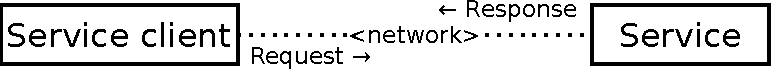
\includegraphics[width=20em]{user_guide/api_sm.pdf}
\end{figure}

\noindent\ignorespaces Our library replaces the \code{\textless{}network\textgreater{}} part. It looks like:
\begin{figure}[H]
\centering
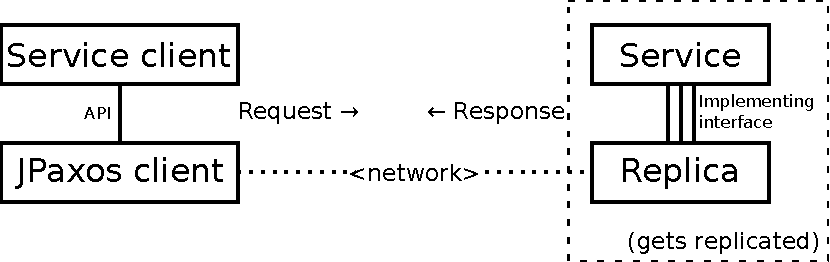
\includegraphics[width=20em]{user_guide/api_jpaxos.pdf}
\end{figure}

In order to make the replication and recovery possible, we require a few additional methods from the Service.

JPaxos provides implementation of it's Client and the Replica. The programmer must implement the Service and make use of the Client class.

\code{Client} sends requests to replicas and waits for reply. It provides only method for connecting and executing requests.

\code{Replica} uses Paxos algorithm to order client requests in all replicas; after deciding requests, executes them on service in proper order. All methods from \code{Service} class are called from one \code{Replica} thread, that means no two will be called concurrently on the service.

\code{Service} executes all requests from clients deterministically. The service must also implement a few additional methods to save and restore its state, which will explained in detail below.

Data exchanged by client and service are in form of byte arrays -- \code{byte{[}{]}}. This gives biggest flexibility to the programmer - any data can be put there. One may use byte arrays in the service, as well as serialise/deserialise the \code{byte{[}{]}} to certain objects.


\subsection{Service}
\label{api:service}
JPaxos provides several base classes and one interface to create a new Service.

The \code{Service} interface, base for all services, describes methods that JPaxos requires from the service to be implemented. \code{Replica} calls all the API methods on the \code{Service} object. To launch the service, one needs to start the governing \code{Replica}.

\clearpage

The inheritance hierarchy is as follows:

\begin{Verbatim}[commandchars=@\[\]]
interface Service
  abstract class AbstractService
    abstract class SimpleService
      abstract class SerializableService
\end{Verbatim}

Using the \code{Service} interface is discouraged in favour of \code{AbstractService}, as the latter implements methods common to all services.

\code{AbstractService} provides widest range of functionality. \code{SimpleService} is the \code{AbstractSer\-vice} narrowed to the absolute minimum for the system to work. \code{Seria\-li\-za\-ble\-Service} differs from \code{SimpleService} only with data type - all client requests and service responses are serialised using Java serialisation.


\paragraphNewline{\texttt{SerializableService} class}
\label{api:serializableservice-class}
This is the simplest class of all available.

This class has minimal number of methods. One requires from the \code{Serializable\-Service} to be able to execute client requests, be able to create a snapshot and roll back to state from a snapshot.

\code{SerializableService} uses Java serialization for creating byte arrays from Object, therefore snapshot, request and reply classes must be serialisable.

Method summary:
\begin{itemize}
\item {} 
\code{abstract Object execute (Object value)}
\begin{quote}

Executes a command from client on this state machine. The return value is sent back to the client.
\end{quote}

\item {} 
\code{abstract Object makeSnapshot ()}
\begin{quote}

Makes snapshot of current Service state. The same data created in this method, will be used to update state from snapshot using \code{updateTo\-Snap\-shot(Object)} method.
\end{quote}

\item {} 
\code{abstract void updateToSnapshot (Object snapshot)}
\begin{quote}

Updates the current state of Service to state from snapshot. This me\-thod will be called after recovery to restore previous state, or if we received newer snapshot from other replica (using catch-up).
\end{quote}

\end{itemize}


\paragraphNewline{\texttt{SimplifiedService} class}
\label{api:simplifiedservice-class}
This class also has minimal number of methods.

Only difference between \code{Simplified\-Ser\-vice} and \code{SerializableService} is the type of passing the data - the \code{SimplifiedService} uses byte arrays for that.

Method summary:
\begin{itemize}
\item {} 
\code{abstract byte{[}{]} execute (byte{[}{]} value)}

\item {} 
\code{abstract byte{[}{]} makeSnapshot ()}

\item {} 
\code{abstract void updateToSnapshot (byte{[}{]} snapshot)}

\end{itemize}


\paragraphNewline{\texttt{AbstractService} class}
\label{api:abstractservice-class}
This class supports three additional functionalities in comparison to \code{Simplified\-Ser\-vice} and \code{SerializableService}:
\begin{itemize}
\item {} 
service may choose when the snapshot has to be done

\item {} 
service may know if the recovery has finished

\item {} 
snapshots can be passed for state after specific request, not only after the last request

\end{itemize}

These features let the service be more flexible and make using threads inside the service code easier. This comes at cost of placing partial responsibility on the service programmer - he must provide valid arguments for the functions.

In order to preserve the functionality, some additional data needs to be remembered by the service.
A sequential number of request identifies each request and request order in JPaxos - these numbers must be taken under consideration in the service as well. This sequential number is global among the replicas.

To make the snapshot creation easier, JPaxos checks the size of logs and previous snapshots. If the ratio between these sizes reaches certain levels (see Configuration chapter) methods \code{askForSnapshot} and \code{forceSnapshot} are called. Programmer should use these methods as hints, although one may just make the snapshot then, or ignore these methods at all.

Method summary:
\begin{itemize}
\item {} 
\code{abstract byte{[}{]} execute (byte{[}{]} value, int executeSeqNo)}
\begin{quote}

Executes the request (\code{value}) and returns the reply for client. The return value must not be null. The \code{executeSeqNo} is the sequential number of this request.
\end{quote}

\item {} 
\code{abstract void askForSnapshot (int lastSnapshotNextRequestSeqNo)}
\begin{quote}

Notifies the service that it would be good to create a snapshot now.
\end{quote}

\item {} 
\code{abstract void forceSnapshot (int lastSnapshotNextRequestSeqNo)}
\begin{quote}

Notifies the service that log is very large and a snapshot should be made.
\end{quote}

\item {} 
\code{final protected void fireSnapshotMade(int nextRequestSeqNo,\\ \indent \hspace{10em} byte{[}{]} snapshot, byte{[}{]} response)}
\begin{quote}

Informs the replica that new snapshot has been made and passes it as the byte array \code{snapshot}. \code{nextRequestSeqNo} is the sequential number of first request that will be executed after the snapshot.

If this method is called from within execute method, after the just executed request, the \code{response} must be also provided (otherwise may be null).
\end{quote}

\item {} 
\code{abstract void updateToSnapshot (int requestSeqNo,\\ \indent \hspace{10em} byte{[}{]} snapshot)}
\begin{quote}

Updates the current state of \code{Service} to the state from the snapshot.
\end{quote}

\item {} 
\code{void recoveryFinished()}
\begin{quote}

Informs the service that the replica is fully functional - i.e. recovery process has been finished (if any).

This implementation is an empty method. One may not override it, if the knowledge that recovery has finished is not needed.
\end{quote}

\end{itemize}


\paragraphNewline{\texttt{Service} interface}
\label{api:service-interface}\label{api:jpaxos-service}
The service interface describes methods that JPaxos requires from the service to be implemented.

Some methods in this interface use \code{SnapshotListener} interface. This interface is very simple, it contains one method only: \code{void onSnapshotMade(int requestSeqNo,\!\linebreak byte{[}{]} snapshot, byte{[}{]} response)}.

This method must be called by \code{Service} when a new snapshot has been made on all previously registered listeners. The parameters match exactly the ones from \code{fire\-Snap\-shot\-Made} method from \code{AbstractService} class.

Method summary:
\begin{itemize}
\item {} 
\code{byte{[}{]} execute (byte{[}{]} value, int executeSeqNo)}

\item {} 
\code{void askForSnapshot (int lastSnapshotNextRequestSeqNo)}

\item {} 
\code{void forceSnapshot (int lastSnapshotNextRequestSeqNo)}

\item {} 
\code{void updateToSnapshot (int requestSeqNo, byte{[}{]} snapshot)}

\item {} 
\code{void addSnapshotListener (SnapshotListener listener)}
\begin{quote}

Registers a new listener. Each listener has to be informed every time a snapshot has been created by \code{Service}.
\end{quote}

\item {} 
\code{void removeSnapshotListener (SnapshotListener listener)}
\begin{quote}

Unregisters the listener.
\end{quote}

\item {} 
\code{void recoveryFinished()}

\end{itemize}


\subsection{Replica}
\label{api:jpaxos-replica}\label{api:replica}
In order to achieve replication above the Paxos protocol another layer must be implemented - a layer that passes the Paxos decisions to the service and accepts client requests. This part is called Replica. Each Replica has one copy of underlying \code{Service}. A replica must have it's unique number - called local Id, or just Id. The Id's are sequential numbers starting from 0.

To create the \code{Replica} object you need:
\begin{itemize}
\item {} 
configuration (shared by replicas and clients)

\item {} 
local Id - identification number

\item {} 
the \code{Service} that has to be replicated

\end{itemize}

The constructor and methods from Replica class are described below:
\begin{itemize}
\item {} 
\code{Replica(Configuration config, int localId, Service service) \\ \indent \hspace{10em} throws IOException}
\begin{quote}

Creates the replica with given \code{Service} and specified Id.

The \code{Configuration} class is described in the {\hyperref[config:jpaxos-configclass]{\emph{Configuration class}}} chapter
\end{quote}

\item {} 
\code{void setLogPath(String path)}
\begin{quote}

Sets path for the logs used by certain crash models. The location of logs must be different for each replica. The path for the logs may also be set in configuration file. However, this method overrides the configuration file setting.

If the log path is set neither in configuration file nor using this method, default \code{jpaxosLogs/\textless{}id\textgreater{}} location is used.
\end{quote}

\item {} 
\code{void start() throws IOException}
\begin{quote}

Starts the replica -- i.e. starts the recovery process and subsequently launches the \code{Service}.
\end{quote}

\end{itemize}


\subsection{Client}
\label{api:jpaxos-client}\label{api:client}
Creating a client is very simple -- each client needs only replica configuration. Then you can easily connect to replicas, and execute commands on them. \code{Client} class takes care of all details related with reconnecting if replica crashes and sending command to other ones.

The Client class has the following methods:
\begin{itemize}
\item {} \begin{description}
\item[{\code{Client() throws IOException}}]
\item[\code{Client(Configuration config) throws IOException}] \hfill

Creates the client. The \code{Configuration} should be the same as for Replica. The first version reads default paxos.properties file, while the latter lets the user choose file location.

\end{description}

\item {} 
\code{void connect()}
\begin{quote}

Connects to the replicates service. This method blocks until the connection will be established.
\end{quote}

\item {} 
\code{synchronized byte{[}{]} execute(byte{[}{]} request)}
\begin{quote}

Executes the request and waits for the response.
\end{quote}

\end{itemize}

\textbf{SerializableClient}

If one chose using \code{SerializableService} as base class for the service implementation, one should use class \code{SerializableClient} rather than \code{Client}. The only difference is that this class deserialises the responses back to objects.


\section{Example: replicated hash map}
\label{example::doc}\label{example:example-replicated-hash-map}
This example presents simple service implementation. The service is a replicated hash map. Each client command reads requested entry and modifies it. Service responds with old map entry value.


\subsection{Service}
\label{example:service}
First, we present an example Service implementation.

\lstset{
language=Java,
basicstyle=\footnotesize\ttfamily,
tabsize=2,
breaklines=true,
breakatwhitespace=false,
lineskip=-0.5em
}

\begin{lstlisting}
    import lsr.service.SimplifiedService;

    public class SimplifiedMapService extends SimplifiedService {

        // Map to be replicated
        private HashMap<Long, Long> map = new HashMap<Long, Long>();

        /** Processes client request and returns the reply for client **/
        @Override
        protected byte[] execute(byte[] value) throws IOException {

            // Deserialise the client command
            MapServiceCommand command;
            command = new MapServiceCommand(value); // this class is not included
            if(!command.isValid())                  // in the example
                return new byte[0];

            // We do the work
            Long oldValue = map.get(command.getKey());
            if (oldValue == null)
                oldValue = new Long(0);
            map.put(command.getKey(), command.getNewValue());

            // We serialise the message back
            ByteArrayOutputStream byteArrayOutput = new ByteArrayOutputStream();
            DataOutputStream dataOutput = new DataOutputStream(byteArrayOutput);
            dataOutput.writeLong(oldValue);

            // And return the reply to the client
            return byteArrayOutput.toByteArray();
        }

        /** Makes snapshot used for recovery and replicas that have very old state **/
        @Override
        protected byte[] makeSnapshot() {
            // In order to make the snapshot, we just serialise the map
            ByteArrayOutputStream stream = new ByteArrayOutputStream();
            try {
                ObjectOutputStream objectOutputStream = new ObjectOutputStream(stream);
                objectOutputStream.writeObject(map);
            } catch (IOException e) {
                throw new RuntimeException("Snapshot creation error");
            }
            return stream.toByteArray();
        }

        /** Brings the system up-to-date from a snapshot **/
        @Override
        protected void updateToSnapshot(byte[] snapshot) {
            // For map service the "recovery" is just recreation of underlaying map
            ByteArrayInputStream stream = new ByteArrayInputStream(snapshot);
            ObjectInputStream objectInputStream;
            try {
                objectInputStream = new ObjectInputStream(stream);
                map = (HashMap<Long, Long>) objectInputStream.readObject();
            } catch (Exception e) {
                throw new RuntimeException("Snapshot read error");
            }
        }
    }
\end{lstlisting}

\subsection{Replica}
\label{example:replica}
In order to run the service, one needs also to write an application starting the service.

\begin{lstlisting}
    public static void main(String[] args) throws IOException {

        /** First, we acquire the ReplicaID **/
        if (args.length > 2) {
            System.exit(1);
        }
        int localId = Integer.parseInt(args[0]);

        /** Then we create the replica, passing to it the service **/
        Replica replica = new Replica(new Configuration(), localId, new SimplifiedMapService());

        /** Then we start the replica **/
        replica.start();

        /** And the service runs until the enter key is triggered **/
        System.in.read();
        System.exit(0);
\end{lstlisting}


\subsection{Client}
\label{example:client}
The code below presents the client side.

\begin{lstlisting}
    import lsr.paxos.client.Client;
    
    (...)
    
    /** Creating the Client object **/
    Client client = new Client();
    client.connect();
    
    (...)
    
    /** Prepairing request **/
    MapServiceCommand command = new MapServiceCommand(key, newValue);
    byte[] request = command.toByteArray();
    
    /** Executing the request **/
    byte[] response = client.execute(request);
    
    /** Deserialising answer **/
    DataInputStream in = new DataInputStream(new ByteArrayInputStream(response));
    
    System.out.println(in.readLong());
\end{lstlisting}


\section{User guide bibliography}
\label{bibliography:bibliography}\label{bibliography::doc}\begin{itemize}
\item {} 
\emph{The part-time parliament}.
L. Lamport.
ACM Transactions on Computer Systems 16, 2 (May 1998), 133-169

\item {} 
\emph{Paxos for System Builders: an overview}.
Kirsch, Jonathan and Amir, Yair.
LADIS `08: Proceedings of the 2nd Workshop on Large-Scale Distributed Systems and Middleware

\item {} 
\emph{Paxos made live: an engineering perspective}.
Chandra, Tushar D. and Griesemer, Robert and Redstone, Joshua.
PODC `07: Proceedings of the twenty-sixth annual ACM symposium on Principles of distributed computing

\end{itemize}

\clearpage

\setcounter{page}{1}
\chapter{Pseudocode of Paxos algorithm}

In this chapter, we present the pseudocode of Paxos algorithm written by us to better understand the algorithm, before writing implementation in Java. The pseudocode was designed and written within IT-SOA project, before the internship at EPFL.

\begin{lstlisting}[frame=lines,caption=Pseudocode of Paxos algorithm]

=================================================
                Classes, structs and data types planned to use
=================================================

/// As process ID we're planning to use a single unsigned int value
typedef uint proc_id;

/// The same counts for decision number
/// The vote_t has also a special value called NULL, set as zero (the votings
/// will begin at least with 1)
typedef uint vote_t;

/// Special "NoVote" value, meaning either no voting, or no earlier promise.
#DEFINE NoVote 0

/// Special value no operation - if all processes having a value are down,
/// we need to ensure no-op will be chosen
#DEFINE NOOP

/// Type for values (which also mean state machine operations)
struct value_t
{
	uint size;
	char * data;
};

/**
 * generic class map assumptions: it's a association table, that means a table
 * indexed by some key. we have [] operator, has value and remove function.
 * At the beginning each map is empty, writing to non-existing element creates
 * it. Some func gives us count.  Most languages have something like that;
 * in C++ it's std::map, in C# it's Dictionary, apparently all descendants
 * of the Map Interface in Java etc.
 **/
template<typename T1, typename T2> class map;


template<typename T1> class set;


/// My process ID - given by joining the group.
proc_id myProcessID = 0;

/**
 * \struct Data
 * Data of the message should contain some value for state machine 
 * and also the client, which send this message. The client is needed
 * because state machine has to know where to send the response to the 
 * message.
 **/
struct Data
{
	char * value;
	Client client;
};

/**
 * \struct Message
 * Proposed representation of the paxos message.
 **/
struct Message
{
	proc_id sender; ///< ID of sending process
	enum messageType ///< Type of the massage
	{
		ALIVE   = 0x00, // For Failure Detector and once used as meaningless message
		PREPARE = 0x01,
		PROMISE = 0x02,
		VOTE    = 0x04,
		VOTED   = 0x08,
		SUCCEED = 0x10,
		NACK    = 0x20, // A not-acknowledge message to make the algorithm faster
		OTHER   = 0xFF, // Yet undefined ;-)
	} type;
	
	uint instanceId; ///< The number of paxos instance
	uint size; ///< Size of the message
	Data data; ///< All the other data 
};

/**
 * \enum Status
 * Indicates the state in which every SinglePaxosEntity currently is.
 **/
enum Status
{
	IDLE,   // the default status of each process
	        // indicates that process try to start new ballot 
	        // (sending prepare messages and waiting for promise responses)

	TRYING, // indicates that process started new ballot
	        // (sending vote messages and waiting for voted responses)

	POLLING 
};

/**
 * \class FailureDetector
 * This class will have current list of all members, with time of 
 * last received message from them. 
 **/
class FailureDetector
{
	public:
		/// By initiating, we do exactly nothing
		FailureDetector(){}
		
		/// Checks, if a process sent anything for the last {timeout} seconds
		isAlive(proc_id id);
		/// Returns lowest process id which is alive
		getLowestAliveId();
		
		/// Class GroupMembers tells the failure detector that the group has
		/// changed
		addMember(proc_id id);
		removedMember(proc_id id);
		
		/// This list holds time of last message from processes, for example as
		/// unix timestamps (seconds elapsed from 01.01.1970)
		map<proc_id, time_t> lastMessageReceived;
		
		/// Time after which a process is thought to be dead
		static const uint timeout;
};


/**
 * \class GroupMembers
 * This class will have current list of all members, that means it will inform
 * whether a process is at that moment taking part in consensus.
 *
 * The list can be modified by the state machine itself, according to the pro-
 * per rules.
 **/
class GroupMembers
{
	public:
		/// Initializes new instance of GroupMembers with specified failure detector.
		/// The specified failure detector will be notified about every change of group 
		/// members.
		///
		/// By initialization we should request group membership; currently we're reading
		/// only a config file.
		GroupMembers(FailureDetector & fd);
	
		list<proc_id> currentMembers;
		isMember(proc_id id);

		addMember(proc_id id); ///< This function also inform failure detector!
		removeMember(proc_id id); ///< This function also inform failure detector!

		getMemberCount();
		getMajority()
	protected:
		FailureDetector & failureDetector;
};

/**
 * \class MessageReceiver
 * Working as a wrapper for incoming messages this class will record time for 
 * every message, check it's type, sender and forward it to Paxos protocol.
 **/
class MessageReceiver
{
	public:
		MessageReceiver(FailureDetector & fd, GroupMembers & gm);
		
		/// Broadcasts message to all members of current group.
		/// Note: This doesn't has to be a reliable broadcast. We cannot
		/// assume that all members will receive this message.
		broadcastMessage(Message msg);
		
		/// Sends message to member with specified id
		sendMessage(proc_id receiver, Message msg);
		
		/// This function will add new listener for incoming messages. The 
		/// listener is function with one argument (message) and returning 
		/// nothing (void). All listeners are executed when new message was
		/// received.
		/// example:
		///   void receiveMessage(Message msg);
		///   messageReceiver.addListener(receiveMessage);
		addListener(function func);
		removeListener(function func);
	protected:
		FailureDetector & failureDetector;
		GroupMembers & groupMembers;
	
		/// This function is designed to receive every message, and after that
		/// forward it if necessary to the Paxos algorithm
		receiveMessage(Message m);
		
		/// The list of all listeners waiting for incoming messages
		list<function> listeners;
};

/**
 * \class MultiPaxos
 * This class is the main class managing whole consensus process.
 * It creates single paxos instances, forwards them appropriate messages etc.
 * If the process is the leader, it must also conduct whole process.
 **/
class MultiPaxos
{
	public:
		MultiPaxos(FailureDetector & fd,
				   MessageReceiver & mr,
				   GroupMembers & gm,
				   StableStorage & ss,
				   StateMachine & sm);
	
		receiveMessage(Message m);
		/// After switching on multiPaxos is informed how many entries had the
		/// file, that is how many entries were read after crash
		fromFile(int how_many_read);
		
		/// Stops current algorithm clearly.
		stop();
	protected:
		FailureDetector & failureDetector;
		MessageReceiver & messageReceiver;
		GroupMembers & groupMembers;
		StableStorage & storage;
		StateMachine & stateMachine;
		
		// The time after which check method will be called in all active paxos instances.
		// static const uint timeout; should be taken from FaliureDetector::timeout
		
		
		/// Determines whether this algorithm is running. This is used to 
		/// stop algorithm clearly.
		bool isRunning;
		
		/// The main loop started in some other thread, used to monitor current
		/// state of single instances. It is important due to crashes of the leader,
		/// and when we have to repeat some paxos algorithm phase. This also fill
		/// not finished instances with NOOP value.
		thread mainLoop
		{
			uint checksPerTimeout = 3;
			run();
		};
		
		/// Gets the process id of current leader. This is lowest id from alive processes
		proc_id getLeader();
		
		/// Determines whether current process is the leader
		bool amILeader();
		
		/// Adds new Paxos instances if necessary; otherwise does nothing
		addMissingPaxos(Message msg)
		
		/// runningPaxos has the list of single Paxos instances started until
		/// this moment. As first message emerges, new instance is created and
		/// added here
		list<SinglePaxosEntity> runningPaxos;
		
		/// The list of instanceId of paxos instances which are not finished yet.
		set<uint> activePaxos;
};

/**
 * \class SinglePaxosEntity
 * Is a single, typical Paxos algorithm. It gets from MultiPaxos only messages
 * for the instance, and takes a single decision.
 **/
class SinglePaxosEntity
{
	public:
		SinglePaxosEntity(StableStorage::SingleEntry my_entry, MessageReceiver & mr, Message msg, uint instanceId)
		receiveMessage(Message msg);
	protected:
		SingleEntry & entry;
		MessageReceiver & messageReceiver;
		
		/// The id of current paxos instance. This is needed to set proper
		/// instance id when sending message to other members (e.g. prepare message)
		uint instanceId;
	
		// The amount of time used to determine whether some phase should be repeated.
		// const uint timeout; should be taken from FaliureDetector::timeout
		
		/// The last time when some message related with specified phase
		/// was received. This times are used to determine whether some 
		/// phase should be repeated
		uint lastTryingTime;
		uint lastPoolingTime;
		
		uint lastMessageTime;
	
		/// This method is called every amount of time, to check crashes.
		/// This is responsible, to start prepare phase if old leader crashes,
		/// and also to repeat some phase if not enough responses is get in 
		/// specified amount of time.
		check(bool amILeader);
	
		/// the methods executed when appropriate message will be received
		prepare(Message & msg);
		promise(Message & msg);
		vote(Message & msg);
		voted(Message & msg);
		succeed(Message & msg);
		
		/// Routine for not acknowledge handling
		nackReceived(Message & msg);
		
		/// Starts the prepare phase, and set current state to TRYING. This 
		/// method sends the prepare message to all processes.
		sendPrepare();
		
		/// Starts the voting phase, and set current state to POOLING. This
		/// method setds the vote message to all processes.
		sendVote();
		
		/// the variables which can be in RAM, and that not a problem if it will
		/// be lost
		
		/// The current status of this paxos instance
		Status status;
		
		/// the set promisers and voters is used by leader only
		
		/// indicates processes from which promise messages was received for lastTriedBallot
		set<proc_id> promisers; 
		/// indicates processes from which voted messages was received for lastTriedBallot
		set<proc_id> voters;
		
		/// The values sent by proccesses in responce to prepare message.
		set<pair<vote_t, value>> valuesSentByPromisers;
		
		/// The message from the client which will be forced when no other process
		/// has some value in first phase.
		Message clientMessage;
};

/**
 * \class StateMachine
 * Represents the state machine. When we run the same state machine on different 
 * processes and execute the same set of methods, in the same order, then on each 
 * process the state machine will be in the same state. This class also manage to
 * check which values can be executed, and when we have to wait for some previous 
 * values.
 */
class StateMachine
{
	public:
		StateMachine(MessageReceiver &  mr);
		
		addValue(Data & data, int instanceId);
		
	protected:
		/// Message receiver used to send response to the client.
		MessageReceiver & messageReceiver;
		
		/// Indicates how many values has been executed on this machine.
		/// This will be always values with numbers from 1 to lastCoherentPart.
		/// Each executed values has to be succeeded in paxos.
		int lastCoherentPart = 0;
		
		/// The data which are currently succeeded on paxos, and are waiting 
		/// to be executed.
		map<int, Data> commands;
		
		/// Executes some data on this state machine.
		execute(Data data);
}

/**
 * \class StableStorage
 * We implement the stable storage as two disk files.
 * One of them has triples of constant-length fields:
 *  - if the consensus succeeded
 *  - last promise value
 *  - last ballot number
 *  - last value number
 *  - offset to the last value
 *  - size of the last value
 * As for the offset: in order to keep files simple, we need to make some
 * easy to implement structure. Thanks to constant length of one entry, we
 * can problemlessly use it without shifting larger part of the file.
 *
 * As for the voting values: initially, they will be empty - we will use any
 * offset for that, and indicate no value with 0 size. As we receive first
 * message with some value, we'll fill offset and size after writing value to
 * the file. Even if we will receive other value (what is a very rare situation
 * because only one process proposes it's value, so we should either accept
 * it, or take an no-op) we can simply by 'loosing' some place skip moving
 * large part of the file. It's acceptable, because we can ensure really small
 * amount of conflicts (in fact, we must do in order to preserve progress).
 **/
class StableStorage
{
	public:
		/// Structure needed by each Paxos instance
		class SingleEntry
		{
			public:
				SingleEntry(uint num, int & offset);
			protected:
				int & lastOffset; /// Reference to value needed for valuesFile
				const number; /// Instance number
				bool succeeded;
				vote_t lastTriedBallot; // The last number of ballot which this process began
				vote_t lastVotedBallot; // The last number of ballot in which this process voted
				vote_t lastPromise; // The last number of ballot which this process promise not to accept lesser one
				int offsetToValue;
				unsigned sizeOfValue;
			public:
				/// The getters simply read value from RAM
				getSucceded() {return succeeded;}
				getLastTriedBallot() {return lastTriedBallot;}
				getLastVotedBallot() {return lastVotedBallot;}
				getLastPromise() {return lastPromise;}
				getValue();
				{return readFile(valuesFile,offsetToValue,size);}

				/// The setters need to write first our function on hard drive
				/// and after then to update RAM
				setSucceded(bool);
				setLastTriedBallot(vote_t);
				setLastVotedBallot(vote_t);
				setLastPromise(vote_t);
				setValue(value_t);
		};

	protected:
		/// Vector (a table) of data stored in RAM for fast read operation
		vector<SingleEntry> paxosData;

		/// Filenames; these need to be constant (or known) in order to allow
		/// crash-recovery. Some configuration file can be later issued
		///
		/// As for pseudocode, these names also indicate open files, that means
		/// writeToFile(mainFile, offset, value) is a allowed write operation.
		/// In real code we'll need at least two variables for this.
		///
		/// stateFile has only number of entries yet initiated;
		/// mainFile has four higher described numbers;
		/// valuesFile has the values.
		///
		/// stateFile is in fact unnecessary, if we can read size of mainFile,
		/// as the record length is constant.
		const string stateFile;
		const string mainFile;
		const string valuesFile;

		int lastOffset;

	public:
		/// In order to simplify the (pseudo)code, we allow to use this class
		/// as typical table of singleEntry objects
		SingleEntry operator[](uint num)
				{ if(paxosData.count()<num) return paxosData[num]; return 0; }

		/// This functions will add objects for new consensus instances
		addNewEntry();
		addNewEntries(int n) { for(n times) addNewEntry();}
		addNewEntriesUpTo(int n) { for( (n-paxosData.count()) times) addNewEntry();}

		/// Returns the number of data == the number of instances
		count() { return paxosData.count(); }

		/// The initializing function must read from file previous data. This
		/// lets crash-recovery; if process crashed, it must read previous
		/// state (if any).
		StableStorage();

};

/**
 * \class Heartbeat
 * This class simply sends every {timeout}/{countPerTimeout} a message treated
 * as 'alive indicator' for all other processes.
 **/
class Heartbeat
{
	public:
		/// This class needs information what group should be informed, and
		/// which class will handle message sending.
		Heartbeat(MessageReceiver & mr, groupMembers & gm);
		
		uint countPerTimeout = 3;
	
	protected:
		list<proc_id> & currentMembers;
		
		MessageReceiver & messageReceiver;
		
		Message mes;
		
		bool isRunning = true;
		
		/// Additional thread OR some scheduling trick is needed in order to
		/// assure the message is sent
		thread heartBeater
		{
			/// Func executed by the thread, here: sending the messagages in
			/// proper moments
			run();
		}
};



==================================================
                                Message handling
==================================================

UPON(receiving message m) execute receiveMessage(Message m) at MessageReceiver

==================================================
                            Pseudo-code of functions
==================================================


-------------------------------------------------
                       Message receiver && failure detector
-------------------------------------------------

MessageReceiver::MessageReceiver(FailureDetector & fd, GroupMembers & gm)
{
	failureDetector = fd;
	groupMembers = gm;
	
	// ### in real implementation we have to implement listening for 
	// ### new incoming messages, and the call receiveMessage
}

MessageReceiver::broadcastMessage(Message msg)
{
	// sending message to all members of current group.
	// 1st way: we iterate through all members of group and send
	// message to them (for TCP protocole)
	// 2nd way: we multicast message (for UDP-multicast)
	
	for(id in gm.currentMembers)
		sendMessage(id, msg);
	OR
	multicast(gm.currentMembers, msg);
}

MessageReceiver::sendMessage(proc_id receiver, Message msg)
{
	// language specific code for sending message
	// it can use some internet protocol like TCP or UDP
	sendMessage(receiver, msg);
}

MessageReceiver::addListener(function func)
{
	listeners.add(func);
}

MessageReveiver::removeListener(function func)
{
	listeners.remove(func);
}
			   
MessageReceiver::receiveMessage(Message m)
{
	// ### check procedure if the message is not from some stupid port scanner
	// ### should go here. As for now, a totally non-byzantine model is assumed


	// If the sender is unknown, we need to check if it isn't in the group
	// (but, in fact, this is unnecessary, the groupMembers should inform
	// us that a new member joined the group
	if ( ! lastMessageReceived.hasKey( m.sender ) )
	{
		if ( ! groupMembers.isMember( m.sender ) )
		{
			drop message;
			return;
		}
	}

	// The last reception time is updated to current system time
	lastMessageReceived[m.sender] = time(0);

	// The type of message is checked, and proper action taken up
	switch ( m.type )
	{
		// If it's heart beat, we should do nothing else
		case ALIVE:
			return;

		// If this is one of consensus messages, we forward it
		case PREPARE | PROMISE | VOTE | VOTED | SUCCEED:
			// notify all listeners about new message
			for(listener in listeners)
				listener(m);
			break;
			
		default:
			// ### If we receive a unknown message, that means something has
			// ### gone wrong - some reaction should be implemented here
	}
}

-------------------------------------------------
							    Failure detector
-------------------------------------------------

FaliureDetector::isAlive(proc_id id)
{
	// the process is suspected to be down when it didn't sent any message
	// in last {timeout} seconds
	return lastMessageReceived[id] - time(0) < timeout;
}

FaliureDetector::addMember(proc_id id)
{
	// We indicate that the process is in group by creating it's slot in map
	// 1st way: we set last time for current time minus timeout - it means
	// we would consider the process for dead. Bad if timeout is't constant
	// (we assume it is)
	// 2nd way: if we use unix time, setting timestamp to 0 would mean setting
	// it to the oldest date we can.
	lastMessageReceived[id] = time(0) - timeout;
	OR
	lastMessageReceived[id] = 0;
}

FaliureDetector::removeMember(proc_id id)
{
	// We simply delete the record. It's even unnecessary to stop tracking
	// this processes (it doesn't take additional time), but many not deleted
	// process id's would mean longer search and bigger memory usage.
	lastMessageReceived.remove(id);
}

FailureDetector::getLowestAliveId()
{
	proc_id lowest = null;
	for(pair<proc_id, time_t> procTime in lastMessageReceived)
	{
		if(lowest == null || lowest > procTime.first)
			lowest = procTime.first;
	}
	return lowest;
}

-------------------------------------------------
						          Multi Paxos
-------------------------------------------------

MultiPaxos::MultiPaxos(FailureDetector & fd,
					   MessageReceiver & mr,
				       GroupMembers & gm,
				       StableStorage & ss,
					   StateMachine & sm);
{
	failureDetector = fd;
	messageReceiver = mr;
	groupMembers = gm;
	storage = ss;
	stateMachine = sm;
	
	// every time there is new message, receiveMessage is executed
	messageReceiver.addListener(receiveMessage);
	
	{ // Here begins recovery process
		Message msg; 
		msg.type = ALIVE;
		msg.instanceId = ss.count(); // We get number of paxoses read from file
		
		addMissingPaxos(msg); // We create the paxoses
		// The main loop will in short time start it's work. It'll automaticly 
		// get all newer values and fill the missing ones.
	}
	
	
	for(int i=1; i<=activePaxos.count(), ++i)
	{
		if(ss[i].getSucceded())
		{
			activePaxos.remove(i);
			stateMachine.addValue(ss[i].getValue());
		}
	}
	
	// start main loop
	isRunning = true;
	
	// Running the main loop thread
	mainLoop.run();
}			   

MultiPaxos::receiveMessage(Message m)
{
	if( ! isRunning) return; // If the algorithm is not running, no message may be forewarded
	
	// is this a message from a client
	if(m is message from client)
	{
		if(m is duplicate message)return;
		
		// if i am not leader I have to send it to current leader
		if(amILeader() == false)
		{
			send(getLeader(), m);
			return;
		}
		m.instanceId = (biggest instanceId from runningPaxos) + 1;
		
		addMissingPaxos(m);
		
		return;
	}
	
	// is this message used by paxos algorithm
	if(m is a paxos message)
	{
		addMissingPaxos(m);
		runningPaxos[m.instanceId].receiveMessage(m);
		
		// if this is succeed message, then we can add this data to state machine
		if(m.messageType == SUCCEED)
		{
			stateMachine.addValue(m.data, m.instanceId);
			activePaxos.remove(m.instanceId);
		}
	}
}

MultiPaxos::addMissingPaxos(Message msg)
{
	// get biggest instance id among running paxos (runningPaxos is a set of numbers)
	uint lastInstanceId = runningPaxos.max();
	
	// If the instance(s) already exist, return
	if(msg.instanceId <= lastInstanceId) return;
	
	
	ss.addNewEntriesUpTo(m.instanceId);
	
	// create all missing paxos
	for(int i = lastInstanceId + 1; i < m.instanceId; i++)
	{
		// message used to initializes paxos instance properly
		Message msg; 
		msg.type = ALIVE;
		msg.instanceId = i;
		
		runningPaxos[i] = new SinglePaxosEntity(ss[i], messageReceiver, msg);
		activePaxos.add(i);
	}
	
	activePaxos.add(m.instanceId);
	runningPaxos[m.instanceId] = new SinglePaxosEntity(ss[m.instanceId], messageReceiver, m);
}

// The starting routine for mainLoop thread
MultiPaxos::mainLoop::run()
{
	while(isRunning)
	{
		bool leader = amILeader();
		foreach(proc_id id, activePaxos)
		{
			runningPaxos[id].check(leader);
		}
		
		// checksPerTimeout is a thread value
		this.suspend( (double) FaliureDetector::timeout / checksPerTimeout);
	}
}

MultiPaxos::amILeader()
{
	return ( getLeader() == myProcessID );
}

MultiPaxos::getLeader()
{
	return failureDetector.getLowestAliveId();
}
		
MultiPaxos::stop()
{
	isRunning = false;
	
	// TODO: Leaving group should go here.
	//       Flushing disk files may also go here
	//       For further implementation.
}
-------------------------------------------------
                               Single Paxos Entity
-------------------------------------------------

SinglePaxosEntity::SinglePaxosEntity(StableStorage::SingleEntry & my_entry, MessageReceiver & mr, Message msg)
{
	entry = my_entry;
	messageReceiver = mr;
	instanceId = msg.instanceId;
	
	clientMessage = 0;
	status = IDLE;
	
	if( msg is a message from client)
	{
		// That means we're the leader
		clientMessage = msg;
		sendPrepare();
	}
	else
	{
		// That means we are not leader, but a typical consensus member
		receiveMessage(msg)
	}
}

SinglePaxosEntity::receiveMessage(Message msg)
{
	// On EVERY message after success, we respond with a succeed message
	// This makes sync possible and faster after we've chosen the value
	if(entry.getSucceded())
	{
		Message succMsg;
		succMsg.messageType = SUCCEED;
		succMsg.instanceId = msg.instanceId;
		succMsg.sender = myProcessID;
		succMsg.data.value = ss.getValue();
		succMsg.size = sizeof(ss.getValue());
		mr.send(msg.sender, succMsg);
	}
	
	lastMessageTime = time(0);
	
	switch(msg.type)
	{
		case ALIVE:      // Used only for initralization of new instnaces
				break;   // for which we got no message yet
		case NACK:
				nackReceived(msg);
				break;
		case PREPARE:
				prepare(msg);
				break;
		case PROMISE:
				promise(msg);
				break;
		case VOTE:
				vote(msg);
				break;
		case VOTED:
				voted(msg);
				break;
		case SUCCEED:
				succeed(mgs);
				break;
		default:
				// some other message which is not handled now
	}
}

SinglePaxosEntity::check(bool amILeader)
{
	if(!amILeader)
	{
		// if i am not the leader, then set status to IDLE. It makes all previous 
		// state not active (like tryig or pooling).
		status = IDLE;
		
		// This means, if nearly for sure the consensus finished, and we don't know this
		if(time(0)-lastMessageTime > 5*FaliureDetector::timeout)
		{
			Message inquiry;
			inquiry.messageType = PREPARE;
			inquiry.instanceId = instanceId;
			inquiry.sender = myProcessID;
			// We cast a prepare for voting no. 0 - a  special no-voting val
			inquiry.data.value = 0;
			inquiry.data.size = sizeof(inquiry.data.value);
			
			mr.send(failureDetector.getLowestAliveId(), inquiry);
		}
	}
	else
	{
		switch(status)
		{
			case IDLE:
				// if we just become a leader, then start prepare phase
				sendPrepare();
				
				break;
			case TRYING:
				// if the prepare phase is too long, then repeat it
				if(time(0) - lastTryingTime > FaliureDetector::timeout)
					sendPrepare();
					
				break;
			case POOLING:
				// if voting phace is too long, then repeat everything from the begining
				if(time(0) - lastPoolingTime > FaliureDetector::timeout)
					sendPrepare();
					
				break;
		}
	}
}


SinglePaxosEntity::nackReceived(Message & msg)
{
	if(msg.ballotNumber != getLastTriedBallot()) return; // Not for this ballot
	if(msg.data.value != status) return; // Not for this phase
	
	switch(status) // We change the times to reinitiate proper round
	{
		case POOLING:
					lastPoolingTime=0;
		case TRYING:
					lastTryingTime=0;
	}
	
	check(true); // We force the instance to check our state, what means
	             // (because of the changed time) restarting some phase
}

SinglePaxosEntity::sendPrepare()
{
	status = TRYING;
	lastTryingTime = time(0);
	
	// we are starting new phase, so we increase the ballot number we start
	entry.setLastTriedBallot(entry.getLastTriedBallot() + 1);
	
	// start prepare phase
	Message prepareMsg;
	prepareMsg.messageType = PREPARE;
	prepareMsg.sender = myProcessID;
	prepareMsg.instanceId = msg.instanceId;
	prepareMsg.data.value = entry.lastTriedBallot();
	prepareMsg.data.value+sizeof(entry.lastTriedBallot)=entry.getValue();
	prepareMsg.size=sizeof(entry.lastTriedBallot)+sizeof(entry.getValue());
	
	messageReceiver.broadcastMessage(prepareMsg);
}

SinglePaxosEntity::sendVote()
{
	// Local atomicity requierd, so that no two local threads
	// will receive messages and get go to this part
	status = POLLING;   
	voters.clear();
	lastPoolingTime = time(0);
	
	if(valuesSentByPromisers.isEmpty())
	{
		// try to force new value from the client
		if( clientMessage == 0 )
		{
			entry.setValue(NOOP);
		}
		else
		{
			entry.setValue( Data(clientMessage.value, clientMessage.sender) );
		}
	}
	else
	{
		// because we receive some value from other proces
		// we have to force it
		
		// We're sorting the values from promisers, the latter as
		// most significant
		// I _do_ know that set must have no order, so in really
		// implementation it will be replaces by something having order.
		sort(valuesSentByPromisers, key, desc);
		// We extract the value from highest voting
		entry.setValue( valuesSentByPromisers->first().value );
	}
	
	// start voting phase
	Message voteMes;
	voteMes.messageType = VOTE;
	voteMes.sender = myProcessID;
	voteMes.instanceId = msg.instanceId;
	voteMes.data.value = entry.lastTriedBallot();
	voteMes.data.value+sizeof(entry.lastTriedBallot)=entry.getValue();
	voteMes.size=sizeof(entry.lastTriedBallot)+sizeof(entry.getValue());
	
	messageReceiver.broadcastMessage(voteMes);
}

SinglePaxosEntity::prepare(Message msg)
{
	// We eliminate the special value, used for getting val from lost consensus
	if(msg.ballotNumber == 0) return;
	
	if(msg.ballotNumber > entry.getLastPromise())
	{
		entry.setLastPromise(msg.ballotNumber);
		lastPromise = msg.ballotNumber;
		
		// response to the leader that we promising to take
		// part in this ballot (we didn't promise to any
		// ballot with higher number yet)
		Message response;
		response.type = PROMISE;
		response.instanceId = instanceId;
		response.sender = myProcessID;
		// If we have any value, we need to append it and its ballot number
		// to the message
		response.data.value=msg.ballotNumber;
		
		response.data.value+sizeof(ballotNumber) = entry.getLastVotedBallot();
		
		response.data.value+sizeof(ballotNumber)+
			sizeof(entry.getLastVotedBallot()) = entry.getValue(); 
		
		response.size = sizeof(ballotNumber)+
			sizeof(entry.getLastVotedBallot())+sizeof(entry.getValue());

		messageReceiver.sendMessage(msg.sender, response);
	}
	else
	{
		// Here we may response that there is ballot with higher
		// voting number
		Message nack;
		nack.messageType = NACK;
		nack.instanceId = msg.instanceId;
		nack.ballotNumber = entry.getLastPromise();
		nack.data.value = POOLING;
		nack.size = sizeof(nack.data.value);
		messageReceiver.sendMessage(msg.sender, nack);
	}
}

SinglePaxosEntity::promise(Message msg)
{
	if(status == TRYING and msg.data.value == entry.getLastTriedBallot())
	{
		// if sender is currently in promisers set then no action is taken,
		// otherwise senders is added to set of promisers
		promisers.union(msg.sender);
		lastTryingTime = time(0);
		
		// We're adding the values given by promisers to some set 
		valuesSentByPromisers.union(pair<msg.data+sizeof(vote_t), msg.data+2*sizeof(vote_t)>);
		
		// if we get promise message from majority of processes, then we can 
		// start sending vote messages
		if(promisers.size() > gm.getMajority())
		{                 
			sendVote();
		}		
	}
}

SinglePaxosEntity::vote(Message msg)
{
	if(entry.getLastPromise() == msg.data.value and msg.data.value > entry.getLastVotedBallot())
	{
		entry.setLastVotedBallot(msg.ballotNumber);
		entry.setValue(msg.data);
		
		// response that we are voting on this ballot
		Message response;
		response.messageType=VOTED;
		response.instanceId=msg.instanceId;
		response.sender=myProcessID;
		response.data.value=msg.ballotNumber;
		response.size=sizeof(msg.ballotNumber);
		
		mr.sendMessage(msg.sender, response);
	}
	else
	{
		// We can send some NACK to inform the leader
		// we already have higher voting number
		Message nack;
		nack.messageType = NACK;
		nack.instanceId = msg.instanceId;
		nack.ballotNumber = entry.getLastPromise();
		nack.data.value = TRYING;
		nack.size = sizeof(nack.data.value);
		messageReceiver.sendMessage(msg.sender, nack);
	}
}

SinglePaxosEntity::voted(Message msg)
{
	if(status == POLLING and msg.data.value == entry.getLastVotedBallot())
	{
		// if sender is currently in voters set then no action is taken,
		// otherwise senders is added to set of voters.
		voters.union(sender);
		lastPoolingTime = time(0);
		
		// if we get the voted message from majority of processes, then we can
		// end by sending succeed message to all processes
		if(voters.size() >= majority)
		{

			Message succMsg;
			succMsg.messageType = SUCCEED;
			succMsg.instanceId = msg.instanceId;
			succMsg.sender = myProcessID;
			succMsg.data.value = ss.getValue();
			succMsg.size = sizeof(ss.getValue());
			
			mr.broadcastMessage(succMsg); //(also to itself)
		}
	}
}

SinglePaxosEntity::succeed(Message msg)
{
	// the order of this operations are very important. If we swap them,
	// it will be possible that we set success value to true, having old
	// value for this instance. After crash we will read that this instance
	// was succeeded, but value will be incorrect.
	setValue(msg.data);
	setSucceeded(true);
}
			   
			   
-------------------------------------------------
                                  State Machine
-------------------------------------------------			   

StateMachine::StateMachine(MessageReceiver & mr)
{
	messageReceiver = mr;
}
			   
StateMachine::addValue(Data & data, int instanceId)
{
	// we can add this data to the list of all finished 
	// consensus data.
	commands[instanceId] = data;
	
	// try to expand the coherent part of commands
	while(commands.containsKey(lastCoherentPart + 1))
	{
		// this to lines should be executed atomic
		execute(commands[lastCoherentPart + 1]);
		lastCoherentPart++;
	}
}

StateMachine::execute(Data data)
{
	// here some action which this state machine do
	print(data.value);
	
	// send respone to client - does everyone send, or only the leader?
	// What if he crashes?
	
	// if(I am the leader)
	// {
		messageReceiver.send(data.klient, ACK);
	// }
}
			   
-------------------------------------------------
                                  Group Members
-------------------------------------------------

GroupMembers::GroupMembers(FailureDetector & fd)
{
	failureDetector = fd;
	
	// group must be formed HERE.
	
	// 1st way:
	// TODO: send a message to join the group
	
	// 2nd way:
	// Read config file
	
	const string groupFile;
	
	int number = 0;
	while ( ! end_of_file(groupFile) )
	{
		currentMembers.add( readFile(groupFile,number) );
		number++;
	}
	
	foreach(proc_id member, currentMembers)
	{
		// We set all the times for now, otherwise we would think we're the leader
		failureDetector.lastMessageReceived[member] = time(0);
	}
	
	// Optional: waiting a timeout for messages to know the group much better at
	// the beginning of consensus.
}

GroupMembers::isMember(proc_id)
{
	return currentMembers.exists(proc_id)
}

GroupMembers::addMember(proc_id id)
{
	// add member to list and notify failure detector
	// that group has changed
	currentMemebers.add(id);
	failureDetector.addMember(id);
}

GroupMembers::removeMember(proc_id id)
{
	// remove member from current members list and notify 
	// failure detector that current group has changed
	currentMembers.remove(id);
	failureDetector.removeMember(id);
}

GroupMembers::getMemberCount()
{
	return currentMembers.size();
}

GroupMembers::getMajority()
{
	return currentMembers.size() / 2 + 1;
}

-------------------------------------------------
                            Stable storage (hard disk)
-------------------------------------------------

StableStorage::SingleEntry::singleEntry(uint num, int & offset)
{
	lastOffset = offset; // warning: both are references!
	number = num; // Entry learns instance number it's offset in main file
	succeeded = false;
	lastBallot = lastPromise = NoVote;
}

StableStorage::SingleEntry::setSucceded(bool s)
{
	writeToFile(mainFile, number*sizeof(singleEntry), s);
	succeeded = s;
}

StableStorage::SingleEntry::setLastBallot(vote_t lb)
{
	writeToFile(mainFile, number*sizeof(singleEntry)+sizeof(succeeded), lb);
	lastBallot=lb;
}

StableStorage::SingleEntry::setLastPromise(vote_t)
{
	writeToFile(mainFile,
			number*sizeof(singleEntry) + sizeof(succeeded) + sizeof(lastBallot),
			lb);
	lastBallot=lb;
}

StableStorage::SingleEntry::setValue(value_t val)
{
	// Two operations here must be done without any other operations on offset
	// value; if one object is not enough for that, one lock should do.
	uint offset = lastOffset;
	lastOffset = lastOffset + val.size;

	writeToFile(valuesFile, offset, val.data.value);

	writeToFile(valuesFile,
				number*sizeof(singleEntry) + sizeof(succeeded) +
				sizeof(lastBallot) + sizeof(lastPromise),
				offset);
	offsetToValue = offset;

	writeToFile(valuesFile,
				number*sizeof(singleEntry) + sizeof(succeeded) +
				sizeof(lastBallot)+sizeof(lastPromise)+sizeof(offsetToValue),
				val.size);
	sizeOfValue = val.size;
	// Only if above one succeeds, the program considers value to be written.


}

StableStorage::SingleEntry::getValue()
{
	if(sizeOfValue == 0) return NULL; // that means a no-value (it's size is 0)
	return readFile(valuesFile,offsetToValue);
}

StableStorage::addNewEntry()
{
	paxosData.add( singleEntry(paxosData.count(), lastOffset) );
	writeToFile(stateFile,0,paxosData.count());
}

StableStorage::StableStorage()
{
	uint count = readFile(stateFile,0, sizeof(uint));

	addNewEntries(count);

	for(count times)
	{
		succeeded = readFile(mainFile, i*sizeof(singleEntry));
		lastPromise = readFile(mainFile, i*sizeof(singleEntry)+...);
		lastBallot = readFile(mainFile, i*sizeof(singleEntry)+...);
		offsetToValue = readFile(mainFile, i*sizeof(singleEntry)+...);
		sizeOfValue = readFile(mainFile, i*sizeof(singleEntry)+...);
	}
}


-------------------------------------------------
                                    Heartbeat
-------------------------------------------------

Heartbeat::Heartbeat(MessageReceiver & mr, groupMembers & gm)
{
	messageReceiver = mr;
	currentMembers = gm.currentMembers;
	
	// Preparing the 'alive' message.
	mes.sender = myProcessID;
	mes.messageType = ALIVE
	mes.instanceId = size = data = NULL; // We don't include these fields here
}

Heartbeat::heartBeater::run()
{
	while(isRunning)
	{
		// Broadcasting the message to others
		mr.broadcastMessage(mes);
		
		// The time _must_be double, otherwise most languages will have 0 in here!
		suspend thread for (double)( FaliureDetector::timeout / countPerTimeout );
	}
}

-------------------------------------------------
                                   Initialization
-------------------------------------------------
// this is example initialization of one multiPaxos instance.
void init()
{
	FailureDetector fd = FailureDetector();
	GroupMembers gm = GroupMembers(fd);
	MessageReceiver msgReceiver = MessageReceiver(fd, gm);
	StableStorage storage = StableStorage();
	MultiPaxos paxos = MultiPaxos(fd, msgReceiver, gm, storage);
}

\end{lstlisting}


\clearpage

% Bibliography (books, articles) starts here.
\pagenumbering{arabic}
\setcounter{page}{\value{pageTemp}}

\bibliographystyle{alpha}{\raggedright\sloppy\small\bibliography{bibliography}}

% Colophon is a place where you should let others know about copyrights etc.
\ppcolophon

\end{document}
